% -----------------------------------------------------------------------------
% -----------------------------------------------------------------------------
%  Universidade Federal do Amazonas
%  Instituto de Computação
%  Ciência da Computação
%
%  Adaptado de pacote abntex2 http://code.google.com/p/abntex2/
%     por Roberto Cidade Fonseca.
% -----------------------------------------------------------------------------
% -----------------------------------------------------------------------------

\documentclass[
	% -- opções da classe memoir --
	12pt,				% tamanho da fonte
	openright,			% capítulos começam em pág ímpar (insere página vazia caso preciso)
	oneside,	
	a4paper,				% tamanho do papel.
	% -- opções da classe abntex2 --
	%chapter=TITLE,		% títulos de capítulos convertidos em letras maiúsculas
	%section=TITLE,		% títulos de seções convertidos em letras maiúsculas
	%subsection=TITLE,		% títulos de subseções convertidos em letras maiúsculas
	%subsubsection=TITLE,	% títulos de subsubseções convertidos em letras maiúsculas
	% -- opções do pacote babel --
	english,				% idioma adicional para hifenização
	brazil				% o último idioma é o principal do documento
]{abntex2/abntex2} % Entre chaves vai o caminho para o arquivo .cls

% ---
% Pacotes básicos
% ---
\usepackage{bookman}				% Usa a fonte Bookman Old Style
\usepackage[T1]{fontenc}			% Selecao de codigos de fonte.
\usepackage[utf8]{inputenc}		% Codificacao do documento (conversão automática dos acentos)
\usepackage{color}				% Controle das cores
\usepackage{graphicx}			% Inclusão de gráficos
\usepackage{microtype} 			% para melhorias de justificação

\usepackage[brazilian,hyper]{backref}	 % Paginas com as citações na bibl
\usepackage[alf]{abntex2cite}	% Citações padrão ABNT
\usepackage{pdfpages} %adicionar documentos pdf. neste caso utilizando no anexo
\usepackage{booktabs} %adicionar tabelas geradas pelo site http://www.tablesgenerator.com
\usepackage[table,xcdraw]{xcolor} %para adicionar cor
\usepackage{multirow} % para adicionar "mesclar" estre células
\usepackage{scalefnt} %definir tamanho da fonte da tabela
\usepackage{verbatim}  %fazer comentários em bloco
\usepackage{float}
\usepackage{subfigure}



\titulo{Uso de técnicas de \textit{Data Mining} na classificação de tipos de dengue}
\autor{Jeferson Barros Alves}
\local{Manaus - AM}
\data{2015}
\orientador[Orientador]{Márcio Palheta Piedade, M.Sc.}
\instituicao{%
  Fundação Centro de Análise, Pesquisa e Inovação Tecnológica
  \par
  Faculdade Fucapi (Instituto de Ensino Superior Fucapi)}
\curso{%
  Coordenação de Graduação em Ciência da Computação}
\tipotrabalho{Monografia}
% O preambulo deve conter o tipo do trabalho, o objetivo, 
% o nome da instituição e a área de concentração 
\preambulo{Monografia apresentada ao Curso de Graduação em Ciência da Computação da Faculdade Fucapi (Instituto de Ensino Superior Fucapi), como requisito parcial para a obtenção do Título de Bacharel em Ciência da Computação. Área de concentração: Banco de Dados.}


% Informações do PDF
\makeatletter
\hypersetup{
    	%pagebackref=true,
	pdftitle={\@title}, 
	pdfauthor={\@author},
    	pdfsubject={\imprimirpreambulo},
    pdfcreator={LaTeX with abnTeX2},
	pdfkeywords={abnt}{latex}{abntex}{abntex2}{trabalho acadêmico},
	bookmarksdepth=4
}
\makeatother

% --- 
% Espaçamentos entre linhas e parágrafos 
% --- 

% O tamanho do parágrafo é dado por:
\setlength{\parindent}{1.3cm}

% Controle do espaçamento entre um parágrafo e outro:
%\setlength{\parskip}{0.2cm}  % tente também \onelineskip

%\setbeforesecskip{3em}
%\setbeforesubsecskip{3em}

% ---
% compila o indice
% ---
\makeindex

% ---------------------------------------------------
% INICIO DE DOCUMENTO
% ---------------------------------------------------

\begin{document}

\noindent

% Seleciona o idioma do documento (conforme pacotes do babel)
%\selectlanguage{english}
\selectlanguage{brazil}

% Retira espaço extra obsoleto entre as frases.
\frenchspacing

% ----------------------------------------------------------
% ELEMENTOS PRÉ-TEXTUAIS
% ----------------------------------------------------------
% \pretextual

% ---
% Capa
% ---
\imprimircapa
% ---

% ---
% Folha de rosto
% (o * indica que haverá a ficha bibliográfica)
% ---
\imprimirfolhaderosto*
% ---
% ---
% Inserir folha de aprovação
% ---
% Isto é um exemplo de Folha de aprovação, elemento obrigatório da NBR
% 14724/2011 (seção 4.2.1.3). Você pode utilizar este modelo até a aprovação
% do trabalho. Após isso, substitua todo o conteúdo deste arquivo por uma
% imagem da página assinada pela banca com o comando abaixo:
%
% \includepdf{folhadeaprovacao_final.pdf}


\begin{folhadeaprovacao}
	\parindent=0pt
	\setlength{\ABNTEXsignskip}{1.5cm}
	
	\begin{center}
		
		%\vspace*{1cm}
		{\fontsize{12}{15}\selectfont\imprimirautor}
		\vspace*{\fill}
		\begin{center}
			\fontsize{12}{15}\selectfont\imprimirtitulo
		\end{center}
		\vspace*{\fill}
	\end{center}	

	Monografia apresentada ao Curso de Graduação em Ciência da Computação da Faculdade Fucapi (Instituto de Ensino Superior Fucapi), como requisito parcial para a obtenção do Título de Bacharel em Ciência da Computação.
	
	Aprovada em:       /      /            , por:

	\assinatura{\fontsize{12}{15}\selectfont Prof. Márcio Palheta Piedade, M.Sc. \\Faculdade Fucapi \\ \fontsize{12}{15}\selectfont \imprimirorientadorRotulo}
	\vspace{1cm}
	\begin{comment}
	\assinatura{\fontsize{12}{15}\selectfont Titulação e nome do(a) membro da banca examinadora \\ \fontsize{11}{15}\selectfont Co-orientador(a), se houver \\ {\fontsize{10}{12}\selectfont Departamento \par Universidade}}
	\vspace{1cm}
	\end{comment}
	\assinatura{\fontsize{12}{15}\selectfont Prof. Sergio Cleger Tamayo, Dr. \\Faculdade Fucapi \\ \fontsize{12}{15}\selectfont Examinador}
	\vspace{1cm}
	\assinatura{\fontsize{12}{15}\selectfont Profa. Marcela Sávia Picanço Pessoa, M.Sc. \\Faculdade Fucapi \\ \fontsize{12}{15}\selectfont Examinadora}
	\vfill
    
	\begin{center}
		\fontsize{12}{15}\selectfont
		\vspace*{0.5cm}
		\imprimirlocal
		\\
		\imprimirdata
		\vspace*{1cm}
	\end{center}
  
 \end{folhadeaprovacao}

% ---
% Dedicatória
% ---
%\begin{dedicatoria}
%   \vspace*{\fill}
%   \noindent
%   \leftskip=5cm
%   Homenagem que o autor presta a uma ou mais pessoas.
%   \vspace{5cm}
%\end{dedicatoria}
% ---
% ---
% Agradecimentos
% ---

\begin{agradecimentos}

Em primeiro lugar quero agradecer a Deus, meu grande amigo, companheiro, e sempre me mostrou o caminho a ser seguido.

A minha  esposa amada  Suzane Barros, que me incetivou nessa jornada.

Ao meu orientador Prof. Márcio palheta, por mostrar-me o caminho da mineração de dados.

Aos meus amigos, Hussama, Wellington, Patrick, Pedro e Tiago que sempre estiveram por perto nesta caminhada.

Agradecimentos também aos que contribuíram de maneira relevante à elaboração deste trabalho, direta ou indiretamente.

\end{agradecimentos}

% ---
% Epígrafe
% ---

%\begin{epigrafe}
%    \vspace*{\fill}
%	\begin{flushright}
%		\textit{Citação}

%		Autor
%	\end{flushright}\vspace{4cm}
%\end{epigrafe}

% ---

% ---
% RESUMOS
% ---

% resumo em português

\setlength{\absparsep}{18pt} % ajusta o espaçamento dos parágrafos do resumo
\begin{resumo}

 	A tarefa de classificação em \textit{Data Mining} consiste na predição de classe dado um determinado conjunto de atributos de uma instância. Esta técnica pode ser útil no diagnóstico médico, como ferramenta de apoio ao profissional da saúde. Na literatura, as melhores técnicas para classificação utilizam máquinas de vetores de suporte e árvore de decisão. Tais técnicas utilizam o conceito de hiperplano para separar de uma melhor forma as classes existentes em conjuntos de dados, também pode-se verificar o uso da divisão e conquista na identificação dos melhores atributos, sendo capazes de produzir resultados mais eficientes no processo de predição. Como resultado, obtivemos modelos classificadores baseados em SMO e J48, que alcançaram resultados de 89,61\% e 86,63\% na classificação correta de instâncias, respectivamente nos conjuntos de dados utilizados neste trabalho, mostrando resultados satisfatórios em relação ao classificador ZeroR utilizando como \textit{baseline}. Foi possível observar também que os modelos gerados obtiveram melhores resultados à medida que os experimentos no tamanho do conjunto de dados aumentava.

 \textit{Palavras-chave}: Mineração de Dados, Classificação, Árvore de Decisão, Bayes, Máquina de Vetor de Suporte.

\end{resumo}

% resumo em inglês

\begin{resumo}[Abstract]
 \begin{otherlanguage*}{english}
   The classification task in \ textit {Data Mining} is the class prediction given a certain set of attributes for an instance. This technique can be useful in medical diagnosis, as a support tool for the health professional. In the literature, the best techniques for classification using support vector machines and decision tree. Such techniques use the concept of hyperplane to separate in a better way the existing classes in data sets, you can also verify the use of divide and conquer to identify the best attributes, being able to produce more efficient results in the prediction process. As a result, we obtained classifiers based models SMO and J48, reaching results of 89.61 \% and 86.63 \% in the correct classification of instances respectively in the data sets used in this study, showing satisfactory results in relation to the classifier Zeror using as \ textit {baseline}. It was also observed that the generated models performed better as the experiments in the data set size increased.

   \vspace{\onelineskip}
 
   \noindent 
   \textit{Keywords}: Data mining, Classifier, Decision Tree, Bayes, Support Vector Machine.
 \end{otherlanguage*}
\end{resumo}

% ---
% inserir lista de figuras
% ---
\pdfbookmark[0]{\listfigurename}{lof}
\listoffigures*
\cleardoublepage
% ---

% ---
% inserir lista de tabelas
% ---
\pdfbookmark[0]{\listtablename}{lot}
\listoftables*
\cleardoublepage
% ---

% ---
% inserir lista de abreviaturas e siglas
% ---
\begin{siglas}
  \item[KDD] \textit{Knowledge Discovery in Databases}
  \item[WEKA] \textit{Waikato Environment for Knowledge Analysis}
  \item[SVM] \textit{Support Vector Machine}
  \item[SMO] \textit{Sequential Minimal Optimization}
  \item[SINAN] Sistema de Informação de Agravos de Notificação
  \item[SUS] Sistema Único de Saúde
\end{siglas}
% ---

% ---
% inserir lista de símbolos
% ---

%\begin{simbolos}
%  \item[$ \lambda $] Lambda
%\end{simbolos}

% ---

% ---
% inserir o sumario
% ---
\pdfbookmark[0]{\contentsname}{toc}
\tableofcontents*
\cleardoublepage
% ---

\textual

\chapter{Introdução}

	Com a grande quantidade de informações geradas e armazenadas por meio do avanço tecnológico das últimas décadas, houve um acúmulo gigantesco de informações. Com isso, surgiram diversas abordagens, técnicas e ferramentas que buscam transformar dados, também conhecida por Descoberta de Conhecimento em Base de Dados (\textit{Knowledge Discovery in Databases - KDD}). Tal abordagem foi proposta em 1989, com o objetivo de analisar os dados de uma base afim de extrair conhecimento útil \cite{fayyad:1996}.	
	
	A computação tem apoiado o desenvolvimento da medicina em diversas áreas como em sistemas de apoio a coleta de dados clínicos e exames por imagens, na organização das informações obtidas, entre outras \cite{costa:2012}. Desta maneira, esse grande volume de dados é uma fonte valiosa de conhecimentos que pode ser utilizada como auxílio ao diagnóstico médico. Com base nisso, é necessário o desenvolvimento de técnicas que permitam a descoberta de conhecimentos em base de dados médicos, para apoiar o médico em sua tarefa diária de tomada de decisões, aumentando a precisão, a confiabilidade e eficiência dos diagnósticos elaborados pelo especialista \cite{costa:2012}.
	
	O número de casos de dengue no Brasil quase triplicou entre 2009 e 2010 segundo dados do Ministério da Saúde. A partir de dados do Ministério da Saúde, mais de um milhão de pessoas podem ter contraído a doença \cite{santos:2011}. Por esta razão observou-se a oportunidade de aplicar técnicas de classificação utilizadas em \textit{Data Minin}, com o objetivo de gerar modelos classificadores com dados oriundos do SINAN (Sistema de Informações de Agravos de Notificação), tendo em vista que o mesmo é utilizado com meio oficial de registro em casos de dengue.
    
    \newpage
	\section{Especificação do problema}
		
		Ao longo dos últimos anos a mineração de dados tem sido cada vez mais utilizada na literatura médica. No entanto, a sua aplicação na análise de dados médicos tem sido relativamente limitada, tendo em vista que a aplicação prática pode explorar o conhecimento disponível no contexto clínico e explicar decisões propostas \cite{bellazzi:2008}. Faz-se importante o desenvolvimento de técnicas que permitam a descoberta de conhecimento em bases de dados médicos, que possam apoiar o profissional em sua tarefa diária de tomada de decisões, aumentando a precisão, a confiabilidade e eficiência dos diagnósticos elaborados pelo especialista \cite{costa:2012}.
		
		Segundo \cite{saude:2013}, a dengue é uma das doenças com maior incidência no Brasil, atingindo a população de todos os estados, independente de classe social. Diante disto, faz-se necessário que um conjunto de ações com intuito de combater os casos de dengue sejam realizadas. Dentre elas temos a previsão de forma antecipada de possíveis novos casos.
		\begin{comment}
		Nesse cenário, torna-se importante que um conjunto de ações para a prevenção da doença seja intensificado, permitindo assim a identificação precoce dos casos de dengue, a tomada de decisões e a implementação de medidas de maneira oportuna a fim de principalmente evitar óbitos.
		\end{comment}
		A classificação epidemiológica dos casos de dengue, que é feita habitualmente após desfecho clínico, na maioria das vezes é retrospectiva, dependendo de informações clínicas e laboratoriais, disponíveis no final do acompanhamento médico. Esses critérios não permitem o reconhecimento precoce de formas potencialmente graves, para as quais é crucial para a instituição de tratamento imediato \cite{saude:2013}.

	\section{Objetivos}
	
		\subsection{Objetivo Geral}

		Construir modelos utilizando as técnicas de classificação em \textit{Data Mining} conhecidas como Árvore de Decisão, \textit{Bayes} e \textit{Support Vector Machine}. Após a criação dos modelos de classificação, avaliar o que obteve melhor resultado em relação ao conjunto de dados utilizados no SINAN (Sistema de Informação de Agravos de Notificação) Dengue do município de Fortaleza. 
		
		\subsection{Objetivos Específicos}
		
		\begin{itemize}
			\item Dividir o conjunto de dados na seguinte quantidade de instâncias: 5.000, 10.000, 15.000, 20.000 e 25.000;
			
			\item Utilizar atributos mais relevantes na tarefa de Classificação;
			
			\item Construir modelos clasificadores com os algoritmos de classificação: J48, REPTree, RandomTree, NaiveBayes e SMO;

			\item Identificar quais modelos gerados possuem melhor desempenho;
			
			\item Validar e interpretar os resultados obtidos no processo de classificação.
		\end{itemize}
		
	\section{Justificativa}
	
	\begin{comment}
	Considera-se a dengue um dos maiores problemas de saúde pública do mundo, especialmente nos países tropicais, cujas condições sócio-ambientais favorecem o desenvolvimento e a proliferação do seu principal vetor o \textsl{Aedes aegypti}. A dengue é, hoje, uma das doenças mais frenquentes no Brasil, atingindo a população em todos os estados, independente de classe social \cite{saude:2008}.
	\end{comment}
	Transmitida pelo mosquito \textit{Aedes aegypti}, a dengue é uma doença viral que se espalha rapidamente pelo mundo. Segundo a Organização Mundial da Saúde (OMS) por volta de 100 milhões de pessoas são infectadas por dengue anualmente, em mais de 100 países, sendo que 2,5 bilhões de pessoas estão sob o risco de infecção, tornando-se assim um dos maiores problemas de saúde pública no mundo \cite{bhatt:2013}. A dengue é, hoje, uma das doenças mais frequentes no Brasil, atingindo a população em todos os estados, independente de classe social \cite{saude:2008}.
	
	Na região das Américas, a doença tem se disseminado com surtos cíclicos ocorrendo a cada 3/5 anos. No Brasil, a transmissão vem ocorrendo de forma continuada desde 1986, intercalando-se com a ocorrência de epidemias, geralmente associadas com a introdução de novos sorotipos em áreas anteriormente não se tinha registro ou alteração do sorotipo predominante. O maior surto no Brasil ocorreu em 2013, com aproximadamente 2 milhões de casos notificados. Atualmente, circulam no país os quatro sorotipos da doença \cite{MS:2015}.
	
	\begin{comment}
	O desenvolvimento de técnicas que permitam a descoberta de conhecimento em bases médicas possui grande importância para apoiar o médico em sua tarefa diária de tomada de decisões, aumentando a precisão, a confiabilidade e a eficiência dos diagnósticos elaborados pelo especialista. 

	Esse apoio computacional pode atuar como uma junta médica virtual, ao trazer para o especialista o conhecimento armazenado em exames e diagnósticos relacionados \cite{costa:2012}.
	\end{comment}
	
	\section{Trabalhos Relacionados}	
	
	No trabalho de \cite{shakil:2015}, observamos que o foco principal do trabalho foi a classificação de dengue, onde inicialmente aplicou-se a classificação nos \textit{datasets} iniciais para identificar qual algoritmo obteve melhor resultado. Os experimentos mostraram que os algoritmos Naive Bayes e J48 obtiveram melhores resultados, onde as maiores contribuições do trabalho foram:
	
	\begin{itemize}
		\item A extração da acurácia de classificação para predição do diagnóstico de dengue.
		\item Comparação de diferentes algoritmos de mineração no conjunto de dados de dengue.
		\item Identificação dos algoritmos com melhor desempenho para previsão dos diagnósticos.
	\end{itemize}
	
	No trabalho de \cite{thitiprayoonwongse:2012}, foi utilizada a técnica de classificação conhecida como Árvore de Decisão \cite{tan:2009}, aplicado a um conjunto de dados temporais contendo dados clínicos e laboratoriais com mais de 400 atributos. Nos experimentos, os dados foram divididos em: conjunto de teste e treinamento, de modo que, o seu objetivo principal foi identificar o dia zero da dengue, pois esta previsão torna-se crítica, tendo em vista que o dia zero tem forte relação com o melhor tratamento do paciente.
	
	No trabalho \cite{santos:2011}, foi desenvolvido um aplicativo para interação dos profissionais da saúde com os dados do SINAN (Sistema de Informação de Agravos de Notificação). Tal aplicativo, escrito em  \textit{Java}\cite{oracle:2015}, implementa algoritmos de classificação e regras de associação da base de dados do SINAN, utilizando o \textit{software} WEKA (\textit{Waikato Environment for Knowledge Analysis}) \cite{weka:2015}. Como resultado, esta ferramenta possibilitou o auxílio no diagnóstico de pacientes.	

	\section{Metodologia de Desenvolvimento}
		
		Com base na metodologia utilizada no processo de Descoberta de Conhecimento em Base de Dados (\textit{Knowledge Dicovery in Databases}) definida em \cite{fayyad:1996}, a realização desta pesquisa será composta das seguintes etapas:
		
		\begin{itemize}
			
			\item A primeira etapa deste trabalho baseado na revisão bibliográfica da literatura relacionada à mineração de dados, para determinar trabalhos relacionados, onde são aplicadas as técnicas de mineração em base de dados médicos para descoberta de conhecimento novo e relevante, que possa auxiliar em diagnósticos do médico especialista;
			
			\item Na segunda etapa, ocorrerá a extração, manutenção e pré-processamento dos dados, onde será realizada a análise  de base de dados para extração de informações de atendimentos de pacientes;
			
			\item Na terceira etapa, será executado algoritmos para descoberta e extração de informações. O objetivo desta etapa será encontrar padrões na base de dados que foi pré-processada, utilizando a ferramenta de mineração WEKA(\textit{Waikato Environment for Knowledge Analysis}), um software \textit{open-source} \cite{opensource:2015} amplamente utilizado por implementar diversos algoritmos de mineração de dados \cite{hall:2009}.
			
			%\item Na primeira etapa, ocorrerá a extração, manutenção e pré-processamento dos dados, onde será realizada a análise de base de dados para extração de informações de atendimentos de pacientes necessários à pesquisa. 
			
			\item Por fim,  na quarta etapa do processo, ocorrerá a análise dos resultados obtidos com a a aplicação dos algoritmos de mineração de dados. Encontrar padrões de classificação que sejam relevantes para a pesquisa em questão.
			
		\end{itemize}
	
	\section{Estruturação da Monografia}
	
		Além deste capítulo introdutório, este trabalho está organizado da forma descrita à seguir. No Capítulo 2, serão descritos conceitos básicos relacionados à compreensão deste trabalho, bem como o referencial teórico. No Capítulo 3, serão apresentados os experimentos juntamente com os resultados obtidos. Finalmente no Capítulo 4, serão apresentadas as conclusões observadas e sugestões de trabalhos futuros da pesquisa.

% ---
% Capítulo 2
% ---
\chapter{Referencial Teórico}

Este Capítulo apresenta uma visão geral dos conceitos envolvidos nas várias técnicas de classificação utilizadas ao longo deste trabalho.

Neste capítulo, apresentamos uma visão geral dos conceitos e procedimentos envolvidos em KDD e consequentemente em Data Mining. Apresentam-se também os trabalhos encontrados na literatura sobre assunto que são relevantes para o desenvolvimento deste trabalho.

	\section{Descoberta de Conhecimento em Base de Dados}
	
	Segundo \cite{fayyad:1996}, a Descoberta de Conhecimento em Base de Dados é um processo não trivial de identificações de novos padrões, válidos e potencialmente úteis.
	
	Em contrapartida, no trabalho de \cite{thome:2002}, define-se KDD como sendo a busca de extração de conhecimento de bases de dados utilizando-se de técnicas e algoritmos que realizam a mineração dos dados para trabalhar e descobrir relações.
	
	O processo de descoberta de conhecimento ocorre quando um conjunto de padrões que são semelhantes, e que podem levar a construção de um modelo. Este processo é formado por 5 etapas: seleção, pré-processamento, transformação, a mineração de dados e a interpretação dos dados \cite{fayyad:1996}. Além do processo, o conhecimento que se deseja buscar deve estar de acordo com três características: deve ser correto, deve ser compreensível para o usuário e deve ter de alguma forma utilidade para o usuário \cite{freitas:2000}.
	
	A seguir serão detalhadas as etapas do processo de KDD de acordo com o apresentado na figura 1.
	
	A etapa de seleção dos dados inicia com a definição do objetivo e mapeamento  dos grupos ou conjuntos de informações que serão utilizados.
	
	O pré-processamento é responsável pelo tratamento de ruídos e dados incompletos.
	
	A transformação tem como objetivo selecionar as principais características que serão utilizadas para representar os dados, ou seja, os dados devem ser selecionados de  modo que sejam os mais úteis para o modelo proposto.
	
	A etapa de mineração de dados é o momento em que serão escolhidos os  algoritmos que mais se ajustam ao objetivo que se quer extrair da base de dados. Além disso, nesta fase são escolhidos os melhores parâmetros para que, no momento do processamento, os resultados sejam os mais rápidos e precisos possíveis.
	
	Ao final do processo teremos a etapa de interpretação e avaliação dos resultados, onde o conhecimento extraído da base de dados é representado por padrões.
\\
		\begin{figure}[h!]
			\caption{\label{figDataMiningFayyad} Etapas do processo KDD.}
			\begin{center}
			    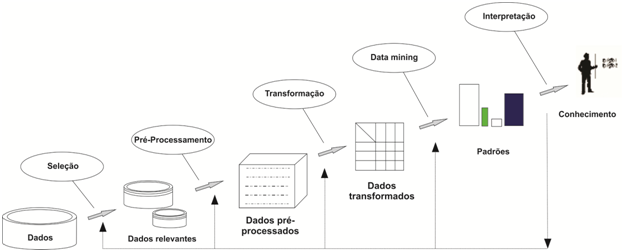
\includegraphics[scale=1]{img/dataMiningFayyad.png}
			\end{center}
			Fonte: Adaptado de \cite{fayyad:1996}.
		\end{figure}
		
		Inicialmente, é necessário definir que tipo de conhecimento se deseja extrair da base de dados, pois a técnica que será utilizada para a mineração de dados depende do objetivo a que se quer chegar \cite{damasceno:2005}.
		
	\section{Data Mining}
	
		Em \cite{berry:1997}, definiu-se \textit{Data Mining} como um processo de exploração e análise, de uma grande quantidade de dados, por meio automático ou semiautomático, com o propósito de descobrir regras e padrões significativos.
		
		É uma técnica que faz parte de uma das etapas da descoberta de conhecimento em banco de dados. É uma área de pesquisa multidisciplinar, incluindo principalmente as tecnologias de banco de dados, inteligência artificial, estatística, reconhecimento de padrões, sistemas baseados em conhecimento, recuperação da informação, computação de alto desempenho e visualização de dados.
		
		Em termos gerais, a técnica de Data Mining compreende os seguintes propósitos:
		
		\begin{itemize}
			\item Previsão – pode mostrar como certos atributos dentro dos dados irão comportar-se no futuro;
			\item Identificação – padrões de dados podem ser utilizados para identificar a existência de um item, um evento ou uma atividade;
			\item Classificação – pode repartir os dados de modo que diferentes classes ou categorias possam ser identificadas com base em combinações de parâmetros;
			\item Otimização do uso de recursos limitados, como tempo, espaço, dinheiro ou matéria-prima e maximizar variáveis de resultado como vendas ou lucros sob um determinado conjunto de restrições.
		\end{itemize}
		
	\subsection{Aprendizagem Não Supervisionada}
	
		Como mostrado por \cite{damasceno:2005} aprendizagem não supervisionada é aquela que utiliza instâncias sem a determinação do atributo classe. Este  tipo de aprendizado é utilizado geralmente para análise exploratória dos dados, utilizando técnicas de  agrupamento ou regras de associação. Onde agrupamentos têm como objetivo relacionar instâncias com características em comuns.
		
		A partir da definição de uma métrica de similaridade, os dados são  agrupados, dando a possibilidade de encontrar relações interessantes entre as instâncias. Assim, o cliente do conhecimento gerado pode aplicar uma determinada ação em um subconjunto de instâncias presente nos  dados. 
		
	\subsection{Aprendizagem Supervisionada}
	
	No aprendizado supervisionado tem-se a figura de um professor externo, o qual apresenta o conhecimento do ambiente por conjuntos de exemplos na forma: entrada, saída desejada. Onde extrai-se a representação do conhecimento a partir desses exemplos. O objetivo é que a representação gerada seja capaz de produzir saídas corretas para novas entradas não apresentadas previametne \cite{lorena:2007}.
	
	\section{Técnicas de Classificação}
	
	Uma técnica de classificação é uma abordagem sistemática para construção de modelos de classificação a partir de um conjunto de dados de entrada. Exemplos incluem classificadores de árvores de decisão, classificadores baseados em regras, redes neurais, máquinas de vetores de suporte e classificadores Bayes simples. Cada técnica emprega um algoritmo de aprendizagem para identificar um modelo que seja mais apropriado para o relacionamento entre o conjunto de atributos e o rótulo da classe dos dados de entrada. O modelos gerado pelo algoritmo de aprendizagem deve se adaptar bem aos dados de entrada e prever corretamente os rótulos de classes de registros que ele nunca viu antes. Portanto, o objetivo chave do algoritmo de aprendizagem é construir modelos com boa capacidade de generalização \cite{tan:2009}.
	
	A Figura \ref{figabordagemModeloClassificacao} mostra uma abordagem geral para resolver problemas de classificação. Primeiro, um conjunto de treinamento consistindo de registros cujos rótulos sejam conhecidos e devem ser fornecidos. O conjunto de treinamento é usado para construir um modelo de classificação, que é subsequentemente aplicado ao conjunto de teste, que consiste de registros com rótulos de classes desconhecidas \cite{tan:2009}.
	\\
	\begin{figure}[!htb]
		\caption{\label{figabordagemModeloClassificacao} Abordagem geral para a construção de um modelo de classificação }
		\begin{center}
			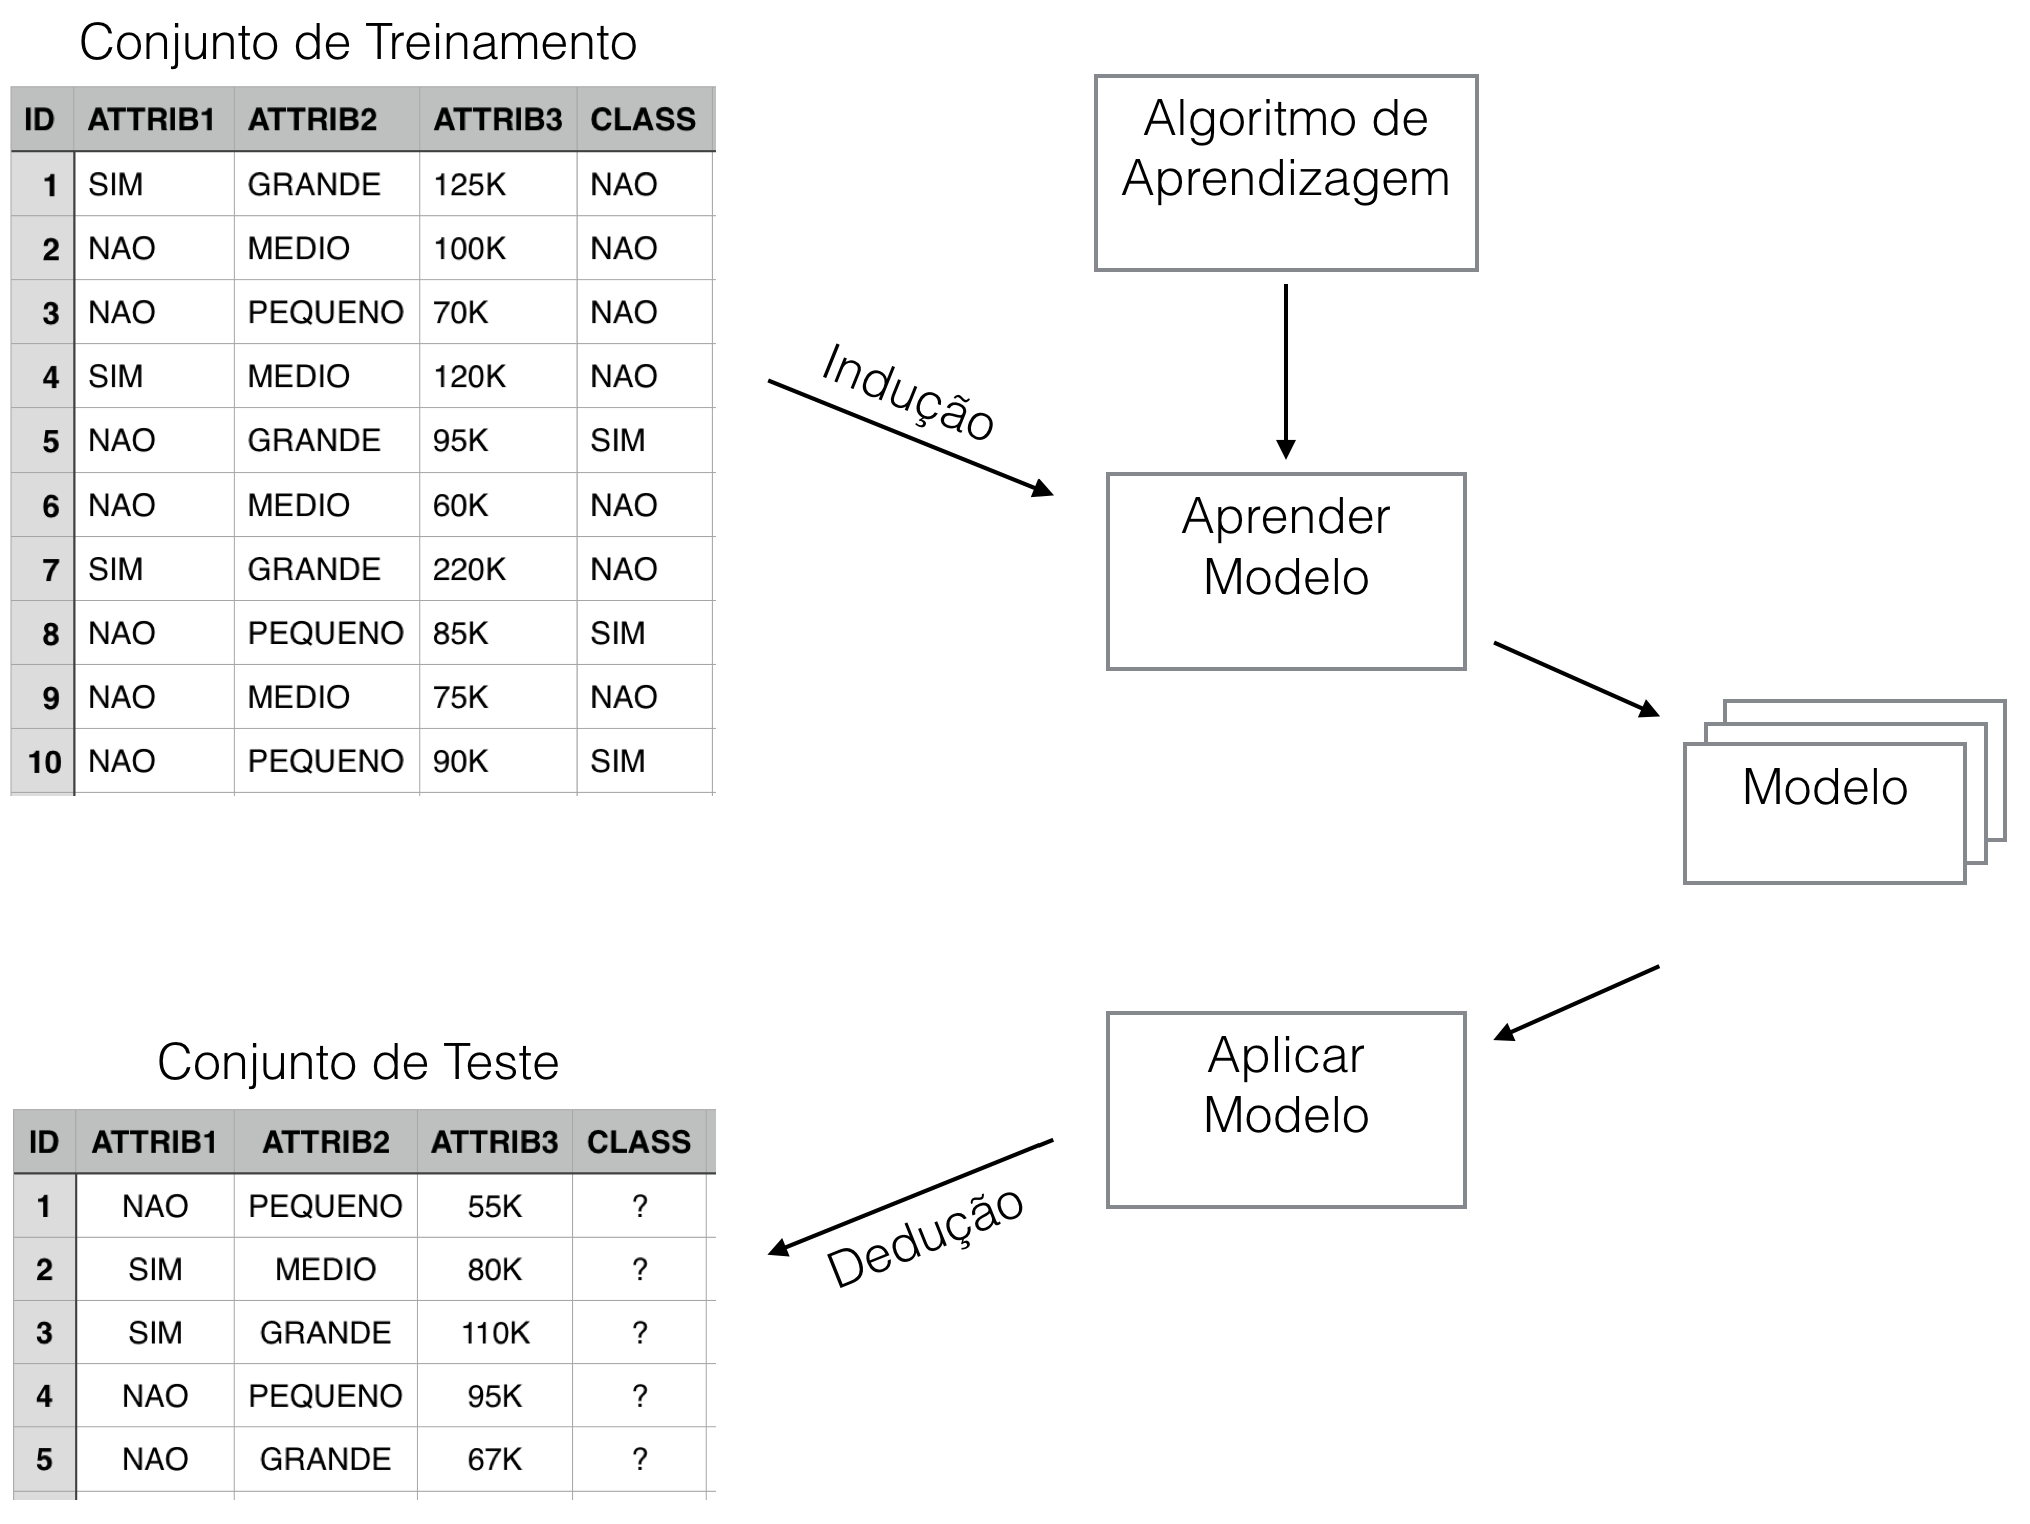
\includegraphics[scale=0.3]{img/abordagemModeloClassificacao.png}
			%			    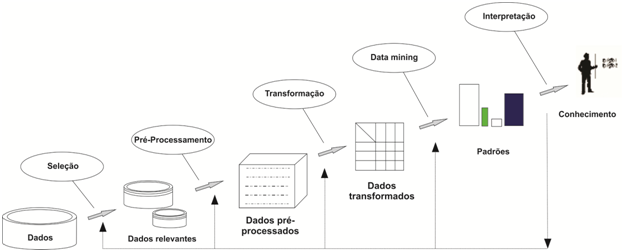
\includegraphics[scale=0.5]{img/dataMiningFayyad}
		\end{center}
		Fonte: Adaptado de \cite{tan:2009}.
	\end{figure}

	\subsection{Árvore de Decisão}
	
		Em uma árvore de decisão, cada nodo folha recebe um rótulo de classe. os nodos não terminais, que incluem o nodo raiz e outros nodos internos, contêm condições de testes de atributos para separar registros que possuem características diferentes.
		
		Classificar um registro de testes é direto, assim que uma árvore de decisão tenha sido construída. Começando do nodo raiz, aplicamos a condição de teste ao registro e seguimos a ramificação apropriada baseados no resultado do teste. Isto nos levará a um outro nodo interno, para o qual uma nova condição de teste é aplicada, ou a um nodo folha \cite{tan:2009}.
	
	\subsubsection{Algoritmo C4.5}
	
	O algoritmo J48 \cite{weka:2015} é uma implementação em Java \cite{oracle:2015} do algoritmo C4.5 \cite{quinlan:94}, que visa gerar árvore de decisão com tratamento de atributos contínuos e discretos, construindo uma árvore com um número de partições variável e com folhas sendo indicadas pelos valores do atributo categórico. 
	
	Segundo \cite{halmenschlager:2002}, para evitar a geração de todas as árvores possíveis, o algoritmo C4.5 se baseia no atributo mais informativo, escolhido entre todos os atributos ainda não considerados no caminho desde a raiz. O algoritmo seleciona como sendo o atributo mais informativo aquele que possuir o maior ganho de informação, resultante da diferença do valor da informação do atributo categórico e do valor da informação (entropia) do atributo em questão.
	
	Para cada atributo é calculado seu ganho de informação. O atributo que tiver o maior valor, será considerado pelo algoritmo como o próximo nodo da árvore. Assim, a partição começa pelo nodo raiz e continua pelos nodos filhos da mesma maneira, até que todos os exemplos desta partição possuam a mesma classe, rotulando-se este nodo como folha e recebendo sua respectiva classe. Na Figura \ref{fignucleoC45}, podemos observar o funcionamento principal do C4.5.
	
		\begin{figure}[!htb]
			\caption{\label{fignucleoC45} Núcleo do Algoritmo C4.5}
			\begin{center}
				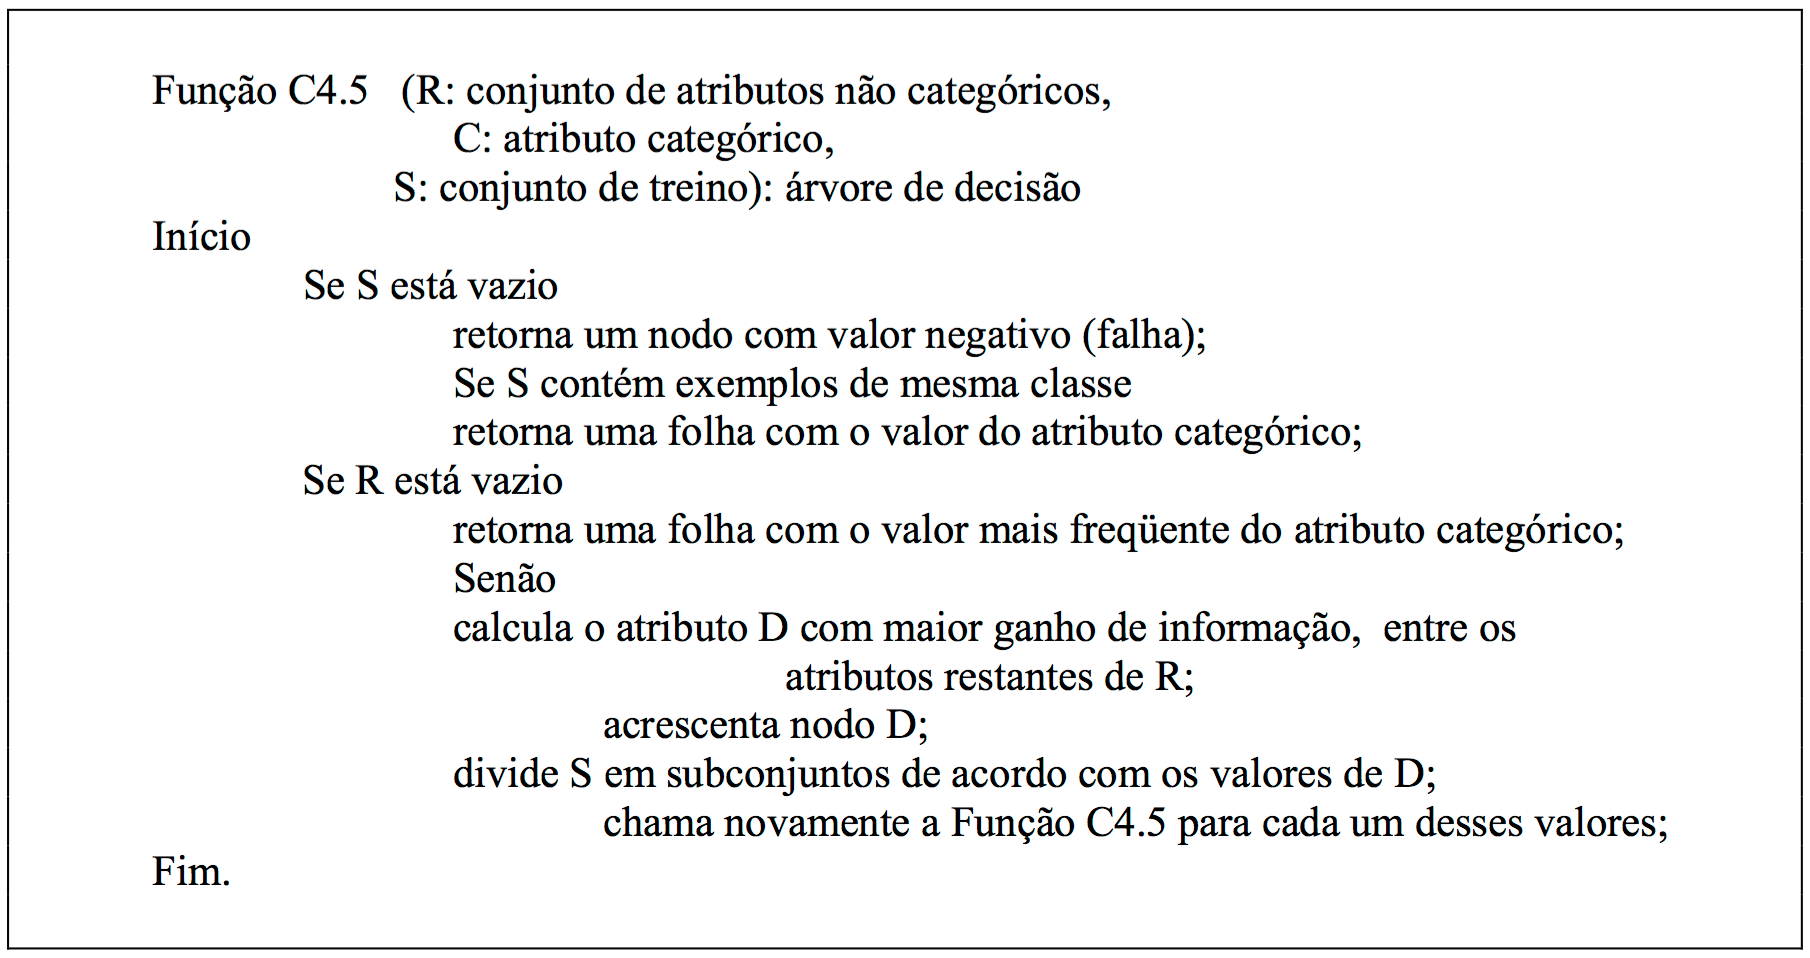
\includegraphics[scale=0.4]{img/nucleoC45.png}
				%			    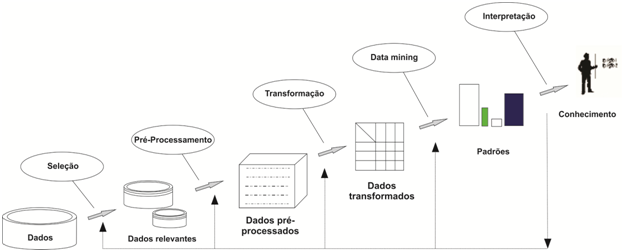
\includegraphics[scale=0.5]{img/dataMiningFayyad}
			\end{center}
			Fonte: \cite{feldens:1997}.
		\end{figure}
	
	O algoritmo recebe o atributo categorico \textit{C} (que indica a classe), um conjunto de atributos não categóricos \textit{R} (demais atributos), e um conjunto de treinamento \textit{S} (que contém os exemplos). Ele verifica qual é o atributo \textit{D} mais informativo de \textit{R}, ou seja, o atributo com maior ganho de informação para o conjunto de treinamento \textit{S} e, então, subdivide este conjunto \textit{S} de acordo com cada um dos valores deste atributo mais informativo \textit{D} \cite{feldens:1997}.
	
	De forma recursiva o algoritmo é chamado para cada subconjunto obtido, até atingir os seguintes objetivos:
	
	\begin{itemize}
		\item Não exista exemplos para classificar o conjunto de treinamento \textit{S}. Neste caso, a árvore de decisão é um nodo com valor negativo;
		\item Que os exemplos no conjunto de treinamento \textit{S} pertençam todos à mesma classe \textit{C}. A árvore de decisão é um folha identificando a classe \textit{$C_i$};
		\item Não exista atributos não categóricos \textit{R} para classificação. A árvore é uma folha identificando a classe \textit{$C_i$} mais frequente de \textit{S}.
	\end{itemize}
	
	Quando o conjunto de treinamentos \textit{S} contém casos pertencentes a várias classes, a ideia é refinar \textit{S} em subconjuntos de casos, que tendem a permanecer em apenas uma classe. A árvore de decisão para \textit{S} consiste de um nodo de decisão que identifica o teste e uma ligação de cada valor possível do atributo. O mesmo processo de construção é aplicado recursivamente em cada subconjunto de casos de treinamento até que a \textit{i-ésima} ligação tenha a árvore de decisão construída do subconjunto \textit{$S_i$} de casos de treinamento. Quando o algoritmo parar, basta percorrer os caminhos desde a raiz até as folhas para verificar as descobertas extraídas da base de dados.
	
	Como observado em \cite{halmenschlager:2002}, os critérios que fazem parte do algoritmo C4.5 são:
	
	\begin{itemize}
		\item Eleição do melhor atributo: utiliza o critério do ganho de informação;
		\item Tratamento dos atributos discretos: atribui uma ligação distinta a cada valor ou forma de agrupamentos de valores em vários conjuntos;
		\item Tratamento de atributos contínuos: Utiliza a técnica do teste simples para partição, escolhendo como ponto de cisão o ponto médio entre os valores;
		\item Tratamento de valores desconhecidos: Desconsidera os atributos com valores deconhecidos, utilizando apenas aqueles com valores totalmente deconhecidos;
		\item Determinação da classe associada à folha: É efetuada por atribuição da classe mais provável nesta folha;
		\item Método de poda: Utiliza a técnica de pós-poda baseada no erro, examinando a árvore de forma \textit{bottom-up} e subtituindo uma subárvore por uma folha;
		\item Complexidade do algoritmo: É dada por \textit{O($mn^{2}$)}, em que \textit{m} é o número de atributos e \textit{n} é o número de instâncias do conjunto de treinamento. 
	\end{itemize}

	\subsubsection{Algoritmo \textit{RandomTree}}
	
	Segundo \cite{oshiro:2013}, considerando um conjunto de treinamento \textit{T} com \textit{a} atributos e \textit{n} exemplos, seja \textit{$T_k$} uma amostra \textit{bootstrap} do conjunto de treinamento a partir de \textit{T} com reposição, contendo \textit{n} exemplos e usando\textit{m} atributos aleatórios \textit{($m\le a$)} em cada nó das árvores.
	
	\textit{RandomTree} é uma árvore induzida aleatoriamente a partir de um conjunto de árvores possíves, usando \textit{m} atributos aleatórios em cada nó. O termo ''aleatoriamente'' significa que cada árvore tem uma chance igual de ser utilizada na amostrada. \textit{Random Trees} podem ser geradas eficientemente e a combinação de grandes conjuntos de \textit{Random Trees} geralmente leva a modelos precisos \cite{zhao:2008}.
	
	\subsubsection{Algoritmo \textit{REPTree}}
	
	O algoritmo \textit{REPTree} constrói árvores de decisão para classificação ou regressão  com base no ganho de informação/variância e poda esta árvore usando uma poda guiada por erro. Otimizado para velocidade, só classifica valores para atributos numéricos uma vez. Os valores são tratadas dividindo as instâncias correspondentes em pedaços (como no algoritmo C4.5) \cite{witten:2011}.
			
	\subsection{Teorema de Bayes}
	
	É um teorema usado para calcular a probabilidade condicional , usando em estatística, probabilidade e outras aplicações
	
	Em muitas aplicações, o relacionamento entre o conjunto de atributos e a variável classe é não determinístico. O rótulo da classe de um registro de teste não pode ser previsto com certeza embora seu conjunto de atributos seja idêntico a alguns dos exemplos de treinamento. Esta situação pode surgir por causa de dados com ruídos ou da presença de determinados fatores de confusão que afetam a classificação mas que não são incluídos na análise.
	
	%Bayes' theorem
	%--------------
	\begin{equation}
		 P(A \mid B) = \frac{P(B \mid A) \, P(A)}{P(B)} 
	\end{equation}
	\\
	Sendo $ P(A\mid B) $ a probabilidade \textbf{posteriori} condicional de A a B, tem-se que:
	\begin{itemize}
		\item $P(B \mid A) $ a probabilidade \textbf{posteriori} condicional de B a A.
		\item $P(A) $ probabilidade \textbf{apriori} de A.
		\item $P(B )$ probabilidade \textbf{apriori} de B.
	\end{itemize}
	
	\subsubsection{Algoritmo NaiveBayes}
	
	O Classificador \textit{NaiveBayes} é uma técnica probabilística baseada no teorema de \textit{Bayes}, expressão, para calcular a probabilidade Posteriori da classe C
	Em \cite{john:1995}
	
	\subsection{Máquinas de Vetores de Suporte (SVM)}
	
	Uma técnica de classificação que tem recebido considerável atenção pois esta técnica possui seus fundamentos na teoria de aprendizagem estatística e tem mostrado resultados empíricos promissores em muitas aplicações práticas, desde o reconhecimento de dígitos escritos à mão até a categorização de textos. SVM também funciona bem com dados de alta dimensionalidade e evita o problema da dimensionalidade. Outro aspecto único desta abordagem é que ela representa o limite da decisão usando um subconjunto dos exemplos de treinamento, conhecido com vetores de suporte \cite{tan:2009}.
	
	Na Figura \ref{figsvmHiperPlanos}, existe um conjunto de classificadores lineares que separam duas classes, mas apenas um (em destaque) que maximiza a margem de separação (distância da instância mais próxima ao hiperplano de separação das classes). O hiperplano com margem máxima é chamado de hiperplano ótimo \cite{junior:2010}.
	
	%\begin{figure}[!htb]
	\begin{figure}[H]
		\caption{\label{figsvmHiperPlanos} Conjunto de hiperplanos possíveis}
		\begin{center}
			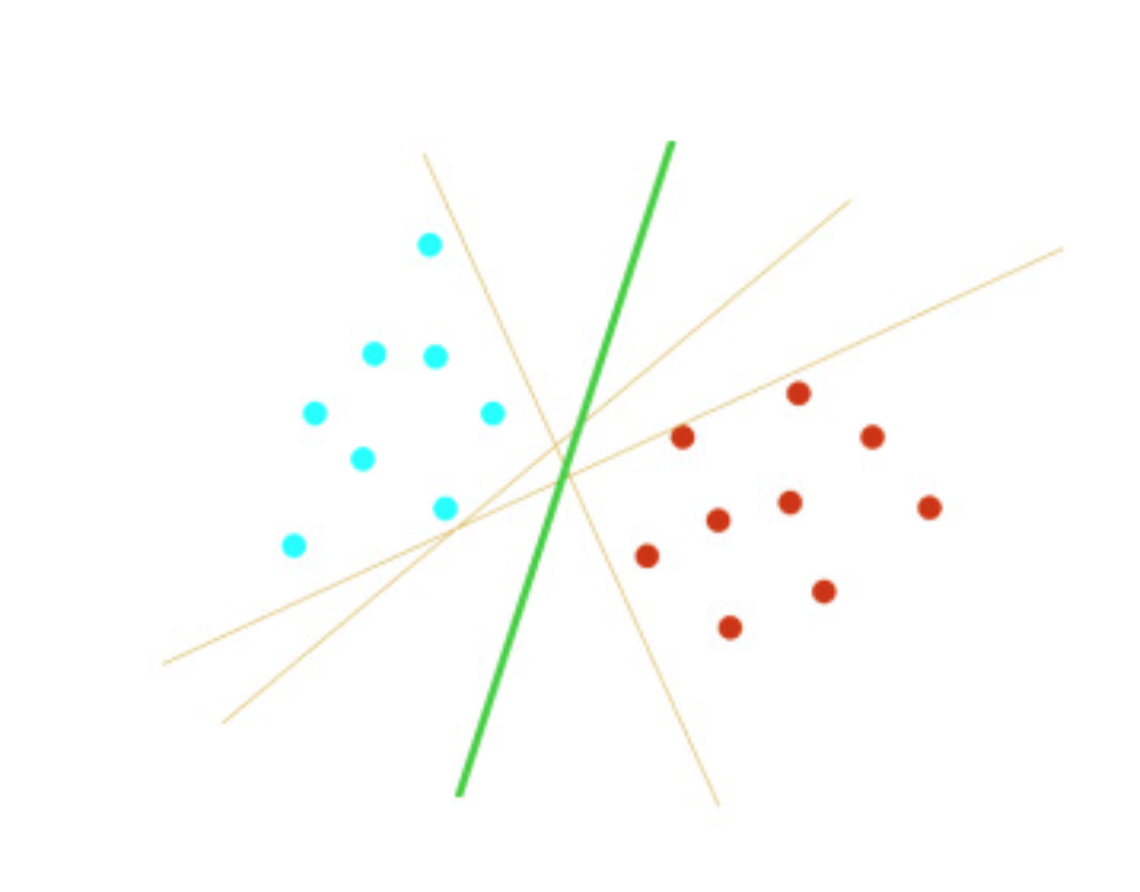
\includegraphics[scale=0.5]{img/svmHiperPlanos.png}
			%			    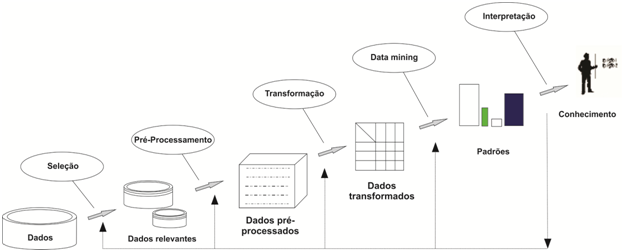
\includegraphics[scale=0.5]{img/dataMiningFayyad}
		\end{center}
		Fonte: \cite{junior:2010}.
	\end{figure}
	
	%\pagebreak
	%\clearpage
	%\newpage
	
	\subsubsection{Algoritmo SMO}
	
	O Algoritmo SMO (\textit{Sequential Minimal Optimization}) \cite{platt:1998}, é um algoritmo simples que pode resolver rapidamente o problema quadrático encontrado em SVM (\textit{Support Vector Machines}) sem qualquer armazenamento extra de matriz e sem o uso de passos de otimização numérica.
	
	O SMO (\textit{Sequential Minimal Optimization}) é um algoritmo de decomposição  que usa uma solução analítica para otimizar um par de Multiplicadores de Lagrange por iteração. Em cada uma delas, três tarefas são executadas: seleção de um par de coeficientes, otimização do par de coeficientes selecionados e atualização de dados globais. A parada do algoritmo ocorre quando todos os coeficientes satisfazem o conjunto de condições. O conjunto de trabalho é formado pelo par de coeficientes a otimizar \cite{hernandez:2009}. 

	\subsection{Métricas para Avaliação de Modelo}
	
	A performance de um modelo de classificação pode ser medida utilizando a matriz de confusão, mostrada na Tabela \ref{tabMatrizConfusao}. Nesta tabela pode ser observado que a distribuição entre as classes (proporção entre exemplos positivos e negativos) é o relacionamento entre a primeira e segunda linha. Assim, qualquer medida de desempenho que utilize valores de ambas as colunas será, necessariamente, sensível a desproporção entre as classes. Havendo mudança na distribuição das classes, os valores das métricas também mudarão, mesmo que o desempenho global do modelo não melhore \cite{prati:2008}.
	\\
	
		\begin{table}[htbp]
			\scalefont{1}
			\centering
			\caption{Matriz de confusão para problemas de classes binárias}
			\label{tabMatrizConfusao}
			\begin{center}
				\renewcommand{\arraystretch}{2}
				\begin{tabular}{ccc}
					\hline
					               & \textbf{Predição positiva}               & \textbf{Predição negativa}         \\ \hline
					\multicolumn{1}{c|}{Classe positiva}                                      & Verdadeiro positivo \textit{(TP)}                                                                                 & Falso negativo \textit{(FN)} 							                                                                                    
					\\
					\multicolumn{1}{c|}{Classe negativa}                                      & Falso positivo \textit{(FP)}                                                                                  &Verdadeito negativo \textit{(TN)} 							                                                                                   							            
					\\ 
					\hline
				\end{tabular}
			\end{center}
			Fonte: Adaptado de \cite{prati:2008}.
		\end{table}
		

		Uma das medidas de desenpenho  mais utilizadas para avaliar a qualidade dos modelos é a \textit{precisão na classificação}, que é definida como $Acc = \frac{TP + TN}{TP + FP + FN + TN} $, ou, equivalente, a \textit{taxa de erro na classificação}, definida como \textit{Err} = 1 - \textit{acc}.
	
		
		\begin{comment}
		\begin{itemize}
			\item \textit{Correctly Classified Instances}: Mostra o percentual de precisão das instâncias corretamente classificados.
			\item \textit{Incorrectly Classified Instances} : Mostra o percentual de precisão das instâncias incorretamente classificados.
			\item \textit{TP Rate}: Taxa de verdadeiros positivos.
			\item \textit{FP Rate}: Taxa de falsos positivos.
			\item \textit{Precision}: Percentual de instâncias positivas classificadas corretamente sobre o total de instâncias classificadas como positivas.
			\item \textit{Recall}: Percentual de instâncias positivas classificadas corretamente sobre o total de instâncias positivas.
			\item \textit{F-Measure}: É uma média ponderada de \textit{Precision} e \textit{Recall}.
			\item \textit{ROC Area}: 
		\end{itemize}
		\end{comment}	

	\section{WEKA (\textit{Waikato Environment for Knowledge Analysis})}
	
	A ferramenta WEKA (Waikato Environment for Knowledge Analysis)  conforme descrito em \cite{hall:2009}, visa proporcionar uma coleção abrangente de algoritmos de aprendizagem de máquina e ferramentas de pré-processamento de dados tanto para pesquisadores como para profissionais. Permite aos usuários experimentar rapidamente e comparar diferentes métodos de aprendizagem de máquina em diferentes conjuntos de dados. Sua arquitetura modular, extensível, permite que os processos de mineração de dados pode ser construido a partir da vasta coleção de algoritmos de aprendizado e diversas ferramentas oferecidas.
		
	\section{Dados Abertos}

	Utilizamos a base de dados disponibilizada pelo portal de dados abertos da prefeitura do Município de Fortaleza de casos notificados de dengue. O portal de dados abertos de Fortaleza é um espaço desenvolvido pela Coordenadoria de Ciência, Tecnologia e Inovação da Prefeitura de Fortaleza (CITINOVA) para que a sociedade possa encontrar e utlizar os dados e informações públicas da cidade de Fortaleza. Os dados são publicados em formatos abertos que permitem sua reutilização em aplicativos digitais desenvolvidos por e para qualquer pessoa. Além disso, o portal serve como uma ferramenta de interlocução com a sociedade fortalezense para pensar e promover  a inovação e a criatividade em prol da melhoria de serviços e da vida na cidade de Fortaleza. O portal de dados abertos de Fortaleza está em conformidade com os princípios da administração pública e observâncias às recomendações aceitas internacionalmente, como as emitidas pela Open Knowledge Foundation e pelo Consórcio W3C Internacional.
		
		
	\section{SINAN}
	
	O Sistema de Informações de Agravos de Notificação (SINAN) é o principal sistema de informações que tem como objetivo os dados referentes a morbidade, sendo fundamental no processo de trabalho da Vigilância em Saúde, estando envolvido não somente nas ações de Vigilância Epidemiológica, mas também na Vigilância Ambiental em Saúde e Vigilância em Saúde do Trabalhador \cite{conass:2015}.
	O SINAN foi desenvolvido no início da década de 90, com o objetivo de padronizar a coleta e o processamento de dados sobre agravos de notificação obrigatória em todo território nacional. Construido de maneira hierarquizada, mantendo coerência com a organização do SUS (Sistem Único de Saúde), pretende ser suficiente ágil na viabilização de análises de situações de saúde em curto espaço de tempo. O SINAN fornece dados para a análise do perfil da morbidade e contribui para a tomada de decisões nos níveis municipal, estadual e federal \cite{saude:2008}.
	A dengue é uma das doenças de notificação compulsória, devendo todo caso suspeito ou confirmado ser notificado ao Serviço de Vigilância Epidemiológica, por meio do SINAN nas fichas de notificação de investigação \cite{saude:2008}.
	
	
% - - -
% Capítulo 3
% - - -
\chapter{Experimentos}

	Neste capítulo, avaliamos os modelos gerados através de uma série de experimentos. Apresentaremos a base de dados utilizada para os experimentos, a metodologia de experimentação e os experimentos em si realizados.

	\section{Base de Dados}
	
	Para avaliar o objetivo geral neste trabalho, usamos a base de dados  do Município de Fortaleza, diposnibilizada pelo portal de dados abertos. Os dados são publicados em formatos abertos que permitem sua reutilização  em aplicativos digitais desenvolvidos por e para qualquer pessoa \cite{fortaleza:2015}. Este conjunto de dados contém notificações de dengue do Município de Fortaleza no período de janeiro à junho de 2015, contendo 26.568 instâncias. %Na Tabela \ref{tabDescricaoAtributos}, podemos observar os atributos utilizados neste trabalho.

\begin{comment}
	\begin{table}[]
		\scalefont{0.6}
		\centering
		\caption{Descrição dos atributos do conjunto de dados}
		\label{tabDescricaoAtributos}
		\begin{tabular}{ll}
			\hline
			Atributos     & Descrição                        \\ \hline
			NU\_NOTIFIC   & Informar a data de investigação  \\
			DT\_NOTIFIC   & Informar ramo da ocupação        \\
			SEM\_NOT      & Informar a classificarão do caso \\
			SG\_UF\_NOT   &                                  \\
			ID\_MUNICIP   &                                  \\
			ID\_REGIONA   &                                  \\
			ID\_UNIDADE   &                                  \\
			SEM\_PRI\_NO  &                                  \\
			MES\_PRIM\_PR &                                  \\
			SEM\_PRI      &                                  \\
			NU\_IDADE\_N  &                                  \\
			NU\_IDADE\_0  &                                  \\
			FX\_NU\_IDADE &                                  \\
			CS\_SEXO &                                  \\
			CS\_GESTANTE &                                  \\
			CS\_RACA &                                  \\
			CS\_ESCOL\_N &                                  \\
			ID\_CNS\_SUS &                                  \\
			SG\_UF &                                  \\
			ID\_MN\_RESI &                                  \\
			ID\_RG\_RESI &                                  \\
			ID\_DISTRIT &                                  \\
			ID\_BAIRRO &                                  \\
			NM\_BAIRRO &                                  \\
			ID\_GEO1 &                                  \\
			NU\_CEP &                                  \\
			DT\_DIGITA &                                  \\
			CS\_FLXRET &                                  \\
			IDENT\_MICR &                                  \\
			DT\_INVEST &                                  \\
			ID\_OCUPA\_N &                                  \\
			DT\_SORO &                                  \\
			RESUL\_SORO &                                  \\
			DT\_NS1 &                                  \\
			RESULT\_NS1 &                                  \\
			DT\_VIRAL &                                  \\
			RESUL\_VI\_N &                                  \\
			DT\_PCR &                                  \\
			RESUL\_PCR\_ &                                  \\
			SOROTIPO &                                  \\
			HISTOPA\_N &                                  \\
			IMUNOH\_N &                                  \\
			CRITERIO &                                  \\
			TPAUTOCTO &                                  \\
			COUFINF &                                  \\
			COMUNINF &                                  \\
			CODSINF &                                  \\
			CO\_BAINF &                                  \\
			NOBAIINF &                                  \\
			DOENCA\_TRA &                                  \\
			EVOLUCAO &                                  \\
			DT\_OBITO &                                  \\
			DT\_ENCERRA &                                  \\
			HOSPITALIZ &                                  \\
			DT\_INTERNA &                                  \\
			UF &                                  \\
			MUNICIPIO &                                  \\
			HOSPITAL &                                  \\
			CLASSI\_FIN   &                                  \\ \hline
		\end{tabular}
		\end{table}
\end{comment}

	\begin{comment}
	Neste Capítulo é descrita a metodologia utilizada para classificação do tipo de dengue em ocorrências do SINAN do município de Fortaleza. Basicamente, pode ser apresentada da seguinte forma:
	\begin{itemize}
		\item Definição de Atributos utilizados: 
		\item Seleção dos Dados:
		\item Particionamento do Conjunto de Dados:
		\item Treinamento dos Classificadores:
	\end{itemize}
	\end{comment}
	
	\section{Pré-processamento}
	\label{Pré-processamento}
	
	Após o download da base de dados em \cite{fortaleza:2015},  iniciamos a importação do arquivo no formato CSV (\textit{Comma Separated Value}), conforme mostrado na Figura \ref{figdataSetOriginal}.
	
		
		\begin{figure}[!htb]
			\caption{\label{figdataSetOriginal} Data Set Original}
			\begin{center}
				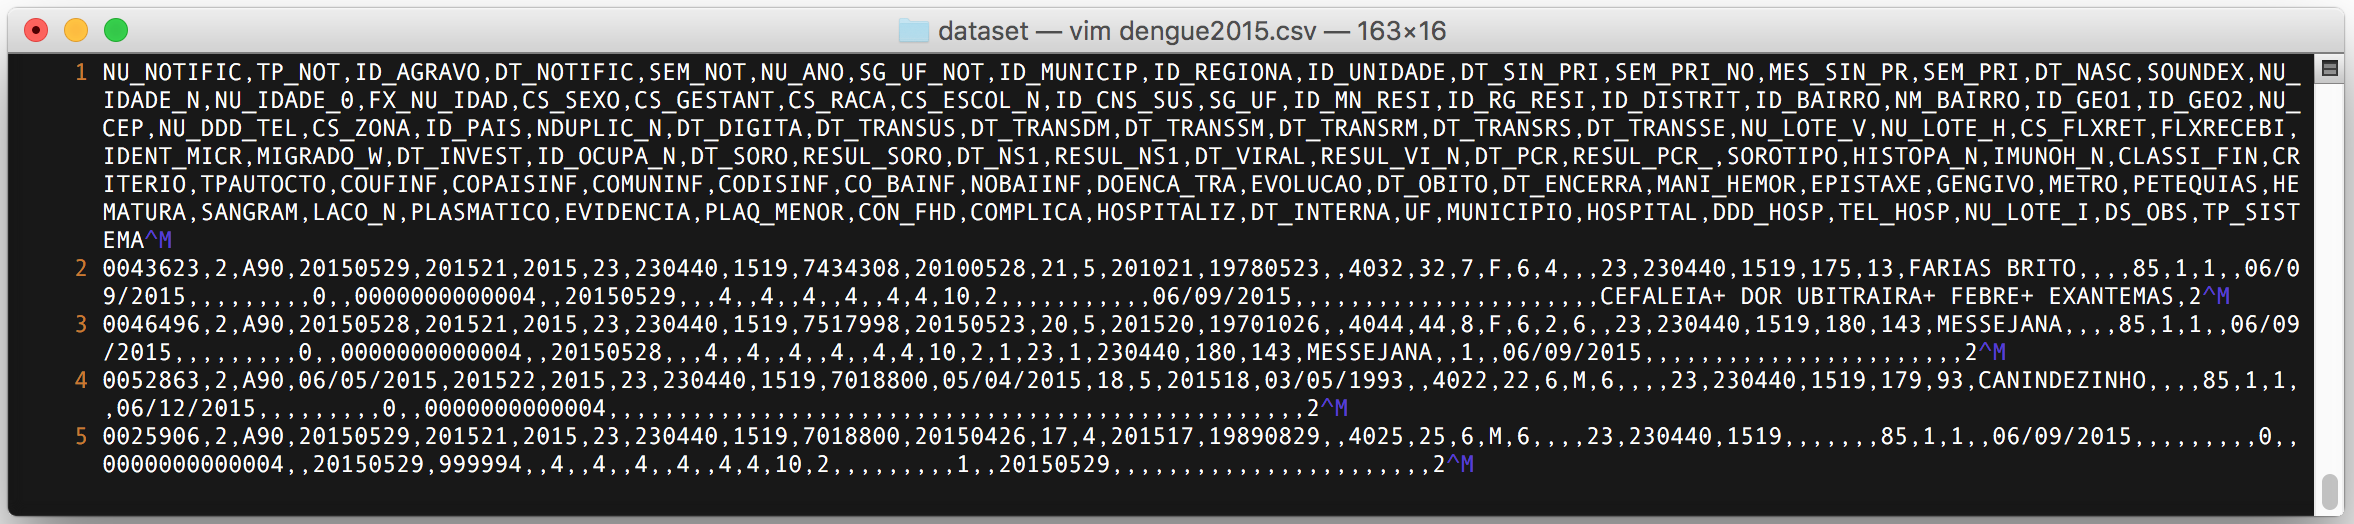
\includegraphics[scale=0.4]{img/dataSetOriginal.png}
			\end{center}
			Fonte: Próprio Autor.
		\end{figure}
	
		\begin{figure}[!htb]
			\caption{\label{figerroCarregarInstancias} Erro ao Carregar Instâncias}
			\begin{center}
				
\includegraphics[scale=0.55]{img/erroCarregarInstancias.png}
			\end{center}
			Fonte: Próprio Autor.
		\end{figure}

	Onde nos deparamos com erros no campos DS\_OBS, onde o WEKA informa que está lendo 102 atributos em vez de 99, conforme mostrado na Figura \ref{figerroCarregarInstancias}. Já na Figura \ref{figerroLinhaSete}, podemos observar que houve falha na inserção dos dados no atributo DS\_OBS, pois o mesmo foi preenchido com vírgula em seu conteúdo da seguinte ''CEFALEIA, FEBRE, DOR NOS OLHOS, VOMITO'', além do caracter ''\^M'' que representa quebra de linha. Pelo fato do arquivo ser contruído no formato CSV (\textit{Comma Separated Value}), essas vírgulas excedentes serão consideradas como início de novos atributos.
	

	
		\begin{figure}[!htb]
			\caption{\label{figerroLinhaSete} Erro Mencionado pelo WEKA}
			\begin{center}
				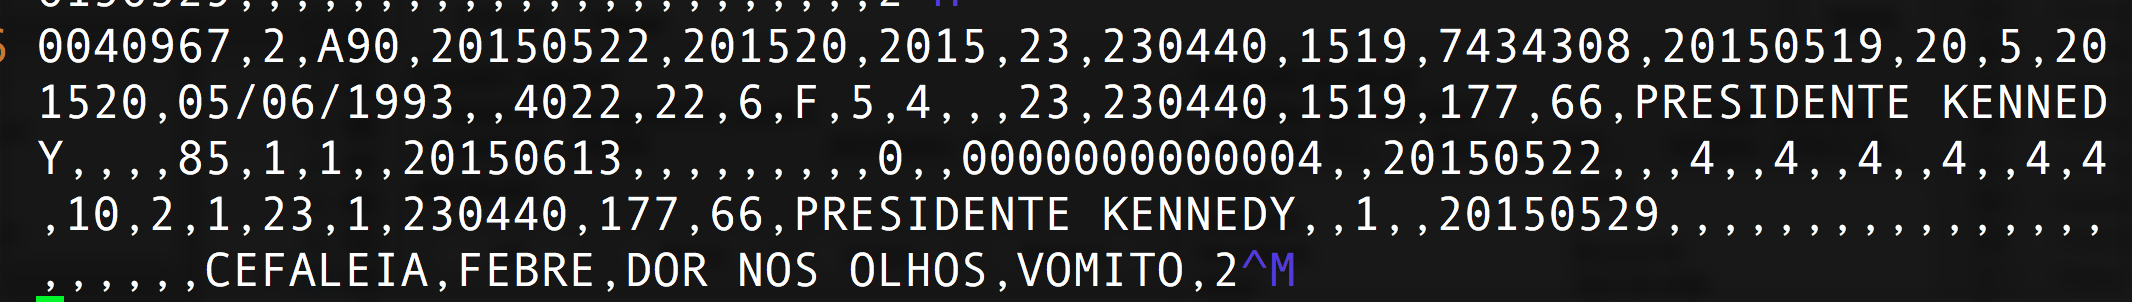
\includegraphics[scale=0.45]{img/erroLinhaSete.png}
			\end{center}
			Fonte: Próprio Autor.
		\end{figure}
		
		Para resolver este problema editamos o arquivo de tal forma que os atributos ''DS\_OBS'' e ''TP\_SISTEMA'' foram removidos. 
		
		Em seguida aplicamos os seguintes filtros:
		
		\begin{itemize}
			\item \textit{RemoveUseless}: Este filtro remove atributos que não variam em tudo ou que variam muito. Todos os atributos constantes são excluídos automaticamente, juntamente com qualquer que exceder o percentual máximo de parâmetro de variação. O teste de variância máxima só é aplicada aos atributos nominais. Utilizamos os parâmetros padrões conforme Figura \ref{figfiltroRemoveUseless}.
			\begin{figure}[!h]
				\caption{\label{figfiltroRemoveUseless} Filtro \textit{RemoveUseless}}
				\begin{center}
					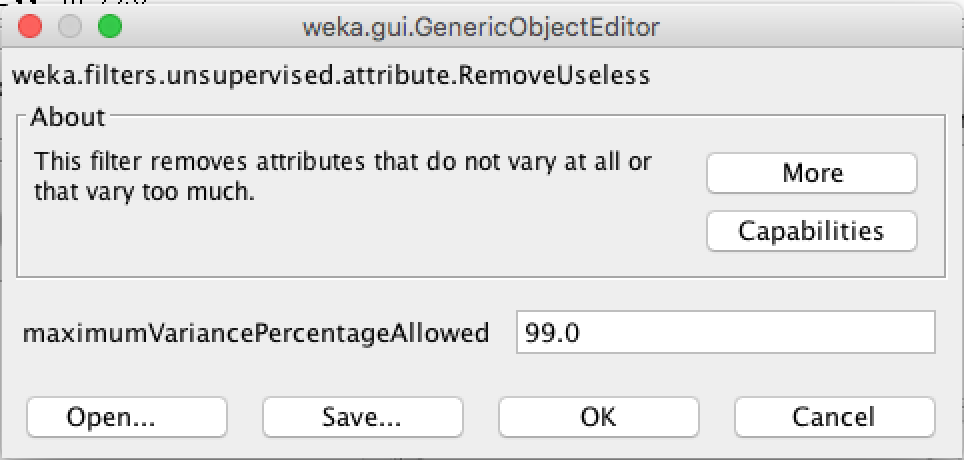
\includegraphics[scale=0.45]{img/filtroRemoveUseless.png}
				\end{center}
				\centering Fonte: Próprio Autor.
			\end{figure}
			\item \textit{NumericToNominal}: Um filtro para transformar numérico atributos em uns nominais. Ao contrário da discretização, apenas toma todos os valores numéricos e os adiciona à lista de valores nominais do que atributo. Útil após a importação CSV, para impor certos atributos para se tornar nominal. Utilizamos o parâmetro mostrado na Figura \ref{figfiltroNumericToNominal}.
			\begin{figure}[!h]
				\caption{\label{figfiltroNumericToNominal} Filtro \textit{NumericToNominal}}
				\begin{center}
					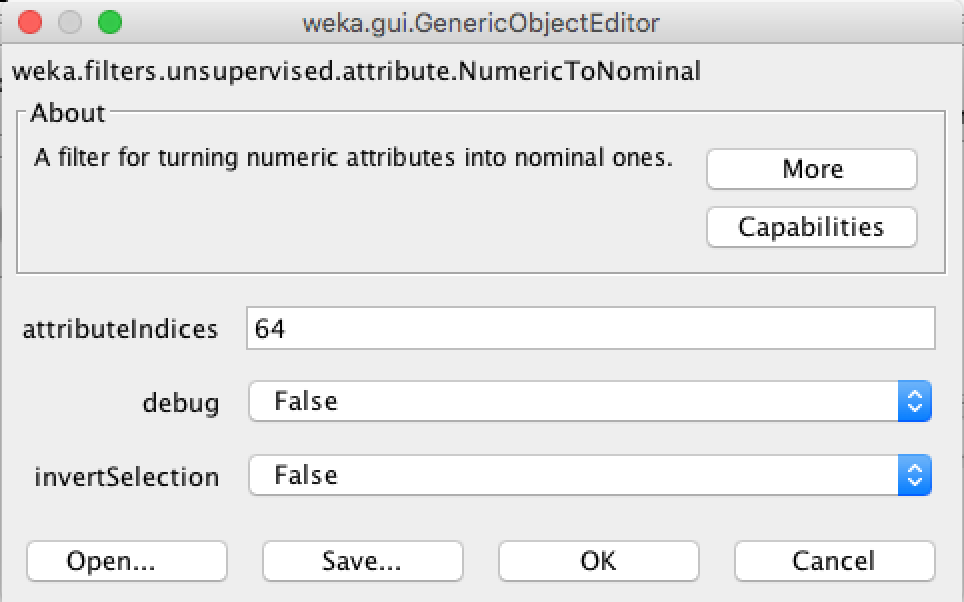
\includegraphics[scale=0.45]{img/filtroNumericToNominal.png}
				\end{center}
				\centering Fonte: Próprio Autor.
			\end{figure}
			\newpage
			\item \textit{RemoveRange}: Um filtro que remove um determinado intervalo de ocorrências de um conjunto de dados. Utilizamos o parâmetro mostrado na Figura \ref{figfiltroRemoveRange}. O parâmetro ''instancesIndices''  foi utilizado cinco vezes para criarmos 05 (cinco) conjuntos de dados com as seguintes quantidades de instâncias: 5.000, 10.000, 15.000, 20.000 e 25.000. Que foram utilizados durantes os experimentos.
			\begin{figure}[!h]
					\caption{\label{figfiltroRemoveRange} Filtro \textit{RemoveRange}}
				\begin{center}
					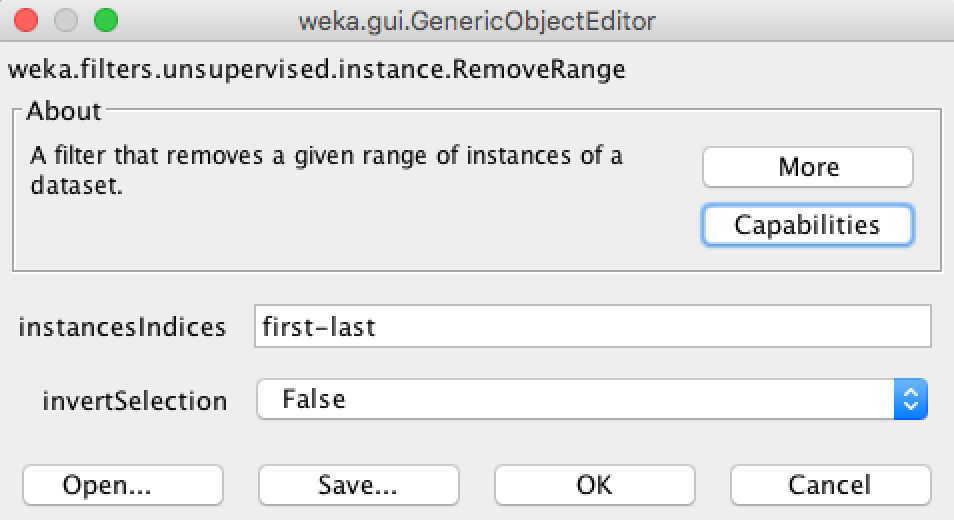
\includegraphics[scale=0.45]{img/filtroRemoveRange.png}
				\end{center}
			\centering Fonte: Próprio Autor.
			\end{figure}
		\end{itemize}

%		$\lambda$
		
	\section{Metodologia do Experimento}
	
	Nossos experimentos foram realizar a partir dos conjuntos de dados divididos nas seguintes quantidades de instâncias: 5.000, 10.000, 15.000, 20.000 e 25.000. A cada conjunto de instâncias, aplicamos os processos de classificação utilizando 5 classificadores que estão contidos em 3 técnicas de classificação, conforme representado na Figura \ref{figmetodologiaExperimentos}. Como resultado dos classificadores obtivemos 25 modelos. 
	
	Todos os testes foram feitos utilizando o processo de validação conhecido como \textit{Cross Validation} diposnibilizado pelo WEKA (\textit{Waikato Environment for Knowledge Analysis}), com o funcionamento da seguinte forma:
	\begin{itemize}
		\item Defini-se o parâmetro \textit{folds}, que utilizaremos com o valor 10;
		\item O conjunto de dados é aleatoriamente reordenado e depois divide-se em conjuntos de tamanho = \textit{folds};
		\item Em cada iteração, um conjunto é usado para testes e os outros \textit{n -1} são utilizados para o treinamento do classificador;
		\item Os resultados do teste são coletados e calculados sobre todos os conjuntos.
	\end{itemize}
	 
	
	\begin{figure}[!htb]
		\caption{\label{figmetodologiaExperimentos} Metodologia Processo dos Experimentos}
		\begin{center}
			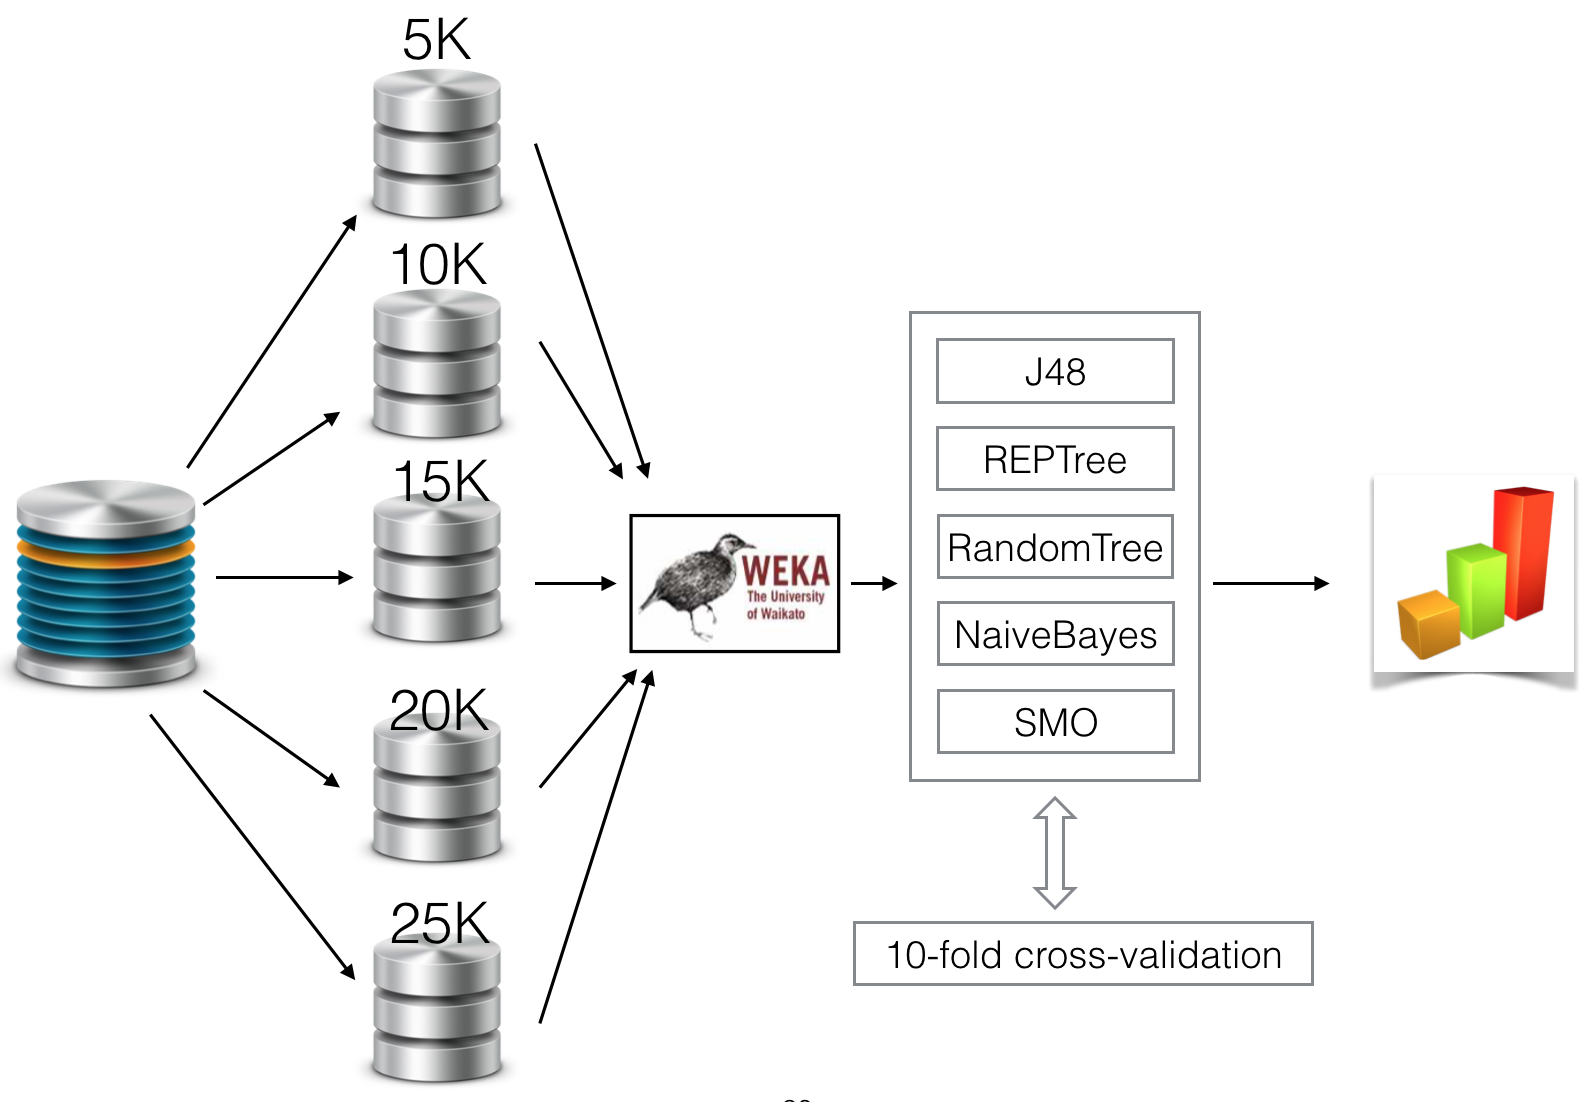
\includegraphics[scale=0.55]{img/metodologiaExperimentos.png}
		\end{center}
		Fonte: Próprio Autor.
	\end{figure}
	
	\section{Resultados}
	
	Nesta seção apresentamos os resultados obtidos na aplicação dos classificadores em  5  conjuntos de dados e as medidas resultantes observadas. Iniciamos o processo de classificação utilizando o conjunto de \textit{datasets} em ordem crescente, que foram  produzidos na Seção \ref{Pré-processamento}. Como resultado obtive-se  as métricas de classificação utilizadas para avaliação da qualidade dos modelos gerados.
	
	\subsection{Precisão na Classificação}
	
	Segundo \cite{witten:2011}, o algoritmo \textit{ZeroR} modela uma base de dados com um única regra. Onde, dado um conjunto de dados para uma nova classificação, o algoritmo prediz o valor mais frequente nos dados de treinamento. Com isso utilizou-se este algoritmo como base de referência para os demais algoritmos utilizados neste trabalho, para que seja possível copará-los entre si.
	
	Na Tabela \ref{tabResultadosClassificacao}, pode-se observar que no \textit{dataset} com 5\textit{k} instâncias o melhor resultado ficou com o algoritmo \textit{SMO} e o pior resultado no algoritmo \textit{ZeroR}. Outro dado importante que pode ser percebido, está relação aos algoritmos: \textit{SMO}, \textit{J48} e \textit{REPTree}. Pois estes algoritmos obtiveram o maior índice de classificação em todos os conjuntos de \textit{datasets}.
	\\
	
	
	% Please add the following required packages to your document preamble:
	% \usepackage{multirow}
	\begin{table}[!htb]
		\scalefont{0.8}
		\centering
		\caption{Resultados de Classificação}
		\label{tabResultadosClassificacao}
		\begin{flushleft}
		\renewcommand{\arraystretch}{2}	
		\begin{tabular}{cccccc}
			\hline
			\multicolumn{1}{c|}{\multirow{2}{*}{\textbf{Classificador}}} & \multicolumn{5}{c}{\textbf{Correctly Classified Instances}}                       \\ \cline{2-6} 
			\multicolumn{1}{c|}{}                                        & 5k instâncias & 10k instâncias & 15k instâncias & 20k instâncias & 25k instâncias \\ \hline
			SMO                                                          & 89,2866\%     & 88,5354\%      & 89,6185\%      & 89,4714\%      & 89,1407\%      \\
			J48                                                          & 86,6530\%      & 86,2315\%      & 86,6322\%      & 85,9331\%      & 85,3096\%      \\
			REPTree                                                      & 83,9683\%     & 79,7414\%      & 80,7076\%      & 79,6344\%      & 77,7052\%      \\
			NaiveBayes                                                   & 83,5592\%     & 76,8103\%      & 76,1682\%      & 74,9666\%      & 70,8689\%      \\
			RandomTree                                                   & 82,0762\%     & 77,2906\%      & 78,8551\%      & 78,0289\%      & 76,6155\%      \\
			ZeroR                                                        & 84,2496\%     & 75,6773\%      & 76,8608\%      & 75,9664\%      & 72,1555\%      \\ \hline
		\end{tabular}
	\end{flushleft}
	\end{table}
	
	\pagebreak
	\clearpage
	%\newpage
	
	\begin{comment}		
		% Please add the following required packages to your document preamble:
		% \usepackage[table,xcdraw]{xcolor}
		% If you use beamer only pass "xcolor=table" option, i.e. \documentclass[xcolor=table]{beamer}
		\begin{table}[htbp]
			\scalefont{1}
			\centering
			\caption{Resultados dos Experimentos com 5.000 instâncias}
			\label{tabResultadosExperimentos5k}
			\begin{center}
	\renewcommand{\arraystretch}{2}
	\begin{tabular}{cp{3cm}p{3.2cm}cc}
		\hline
		\textbf{Classificador}                & \textbf{Correctly Classified Instances}               & \textbf{Incorrectly Classified Instances}      	& \textbf{TP Rate}						&\textbf{FP Rate}   \\ \hline
		SMO                                      & 89,2866\%                                                                                 & 10,7134\% 							&0.863									&0.346                                                                                    \\
		J48                                      & 86,6530\%                                                                                  & 13,3470\% 							&0.867										&0.701                                                                                     \\
		REPTree                                  & 83,9683\%                                                                                 & 16,0317\%								&0.84											&0.815                                                                                     \\
		NaiveBayes                               & 83,5592\%                                                                                 & 16,4408\%								&0.836												&0.619                                                                                     \\ \hline \hline
		ZeroR    									& 84,2496\%                                                 									& 15,7504\%								&0.842											&0.842                                                     								\\
		RandomTree                               & 82,0762\%                                                                                 & 17,9238\%									&0.821												&0.623                                                                                     \\ \hline
	\end{tabular}
\end{center}
\end{table}
		
		
				\begin{table}[htbp]
					\scalefont{1}
					\centering
					\caption{Resultados dos Experimentos com 10.000 instâncias}
					\label{tabResultadosExperimentos10k}
					\begin{center}
						\renewcommand{\arraystretch}{2}
						\begin{tabular}{cp{3cm}p{3.2cm}cc}
							\hline
							\textbf{Classificador}                & \textbf{Correctly Classified Instances}               & \textbf{Incorrectly Classified Instances}      	& \textbf{TP Rate}						&\textbf{FP Rate}   \\ \hline
							SMO                                      & 88.5345\%                                                                                 & 11.4655\% 							&0.885									&0.218                                                                                    \\
							J48                                      & 86,2315\%                                                                                  & 13,7685\% 							&0.862										&0.328                                                                                     \\
							REPTree                                  & 79,7414\%                                                                                 & 20,2586\%								&0.797											&0.497                                                                                     \\
							RandomTree                               & 77,2906\%                                                                                 & 22,7094\%								&0.773												&0.408                                                                                     \\
							NaiveBayes    									& 76,8103\%                                                 									& 23,1897\%								&0.768											&0.420                                                     								\\ \hline \hline
							ZeroR                               & 75,6773\%                                                                                 &  24,3227\%									&0.757												&0.757                                                                                     \\ \hline
						\end{tabular}
					\end{center}
				\end{table}
		
		
\begin{table}[htbp]
	\scalefont{1}
	\centering
	\caption{Resultados dos Experimentos com 15.000 instâncias}
	\label{tabResultadosExperimentos15k}
	\begin{center}
		\renewcommand{\arraystretch}{2}
		\begin{tabular}{cp{3cm}p{3.2cm}cc}
			\hline
			\textbf{Classificador}                & \textbf{Correctly Classified Instances}               & \textbf{Incorrectly Classified Instances}      	& \textbf{TP Rate}						&\textbf{FP Rate}   \\ \hline
			SMO                                      & 89,6195\%                                                                                 & 10,3805\% 							&0.896									&0.207                                                                                    \\
			J48                                      & 86,6322\%                                                                                  & 13,3678\% 							&0.866										&0.335                                                                                     \\
			REPTree                                  & 80,7076\%                                                                                 & 19,2924\%								&0.807											&0.507                                                                                     \\ \hline \hline
			ZeroR                               & 76,8608\%                                                                                 & 23,1392\%								&0.769												&0.769                                                                                     \\
			RandomTree    									& 78,8551\%                                                 									& 21,1449\%								&0.789											&0.435                                                     								\\ 
			NaiveBayes                               & 76,1682\%                                                                                 &  23,8318\%									&0.762												&0.448                                                                                     \\ \hline
		\end{tabular}
	\end{center}
\end{table}		


\begin{table}[htbp]
	\scalefont{1}
	\centering
	\caption{Resultados dos Experimentos com 20.000 instâncias}
	\label{tabResultadosExperimentos20k}
	\begin{center}
		\renewcommand{\arraystretch}{2}
		\begin{tabular}{cp{3cm}p{3.2cm}cc}
			\hline
			\textbf{Classificador}                & \textbf{Correctly Classified Instances}               & \textbf{Incorrectly Classified Instances}      	& \textbf{TP Rate}						&\textbf{FP Rate}   \\ \hline
			SMO                                      & 89,4714\%                                                                                 & 10,5286\% 							&0.895									&0.199                                                                                    \\
			J48                                      & 85,9331\%                                                                                  & 14,0669\% 							&0.859										&0.324                                                                                     \\
			REPTree                                  & 79,6344\%                                                                                 & 20,3656\%								&0.796											&0.499                                                                                     \\ 
			RandomTree                               & 78,0289\%                                                                                 & 21,9711\%								&0.780												&0.426                                                                                     \\ \hline \hline
			ZeroR    									& 75,9664\%                                                 									& 24,0336\%								&0.760											&0.760                                                     								\\ 
			NaiveBayes                               & 74,6696\%                                                                                 &  25,3304\%									&0.747												&0.417                                                                                     \\ \hline
		\end{tabular}
	\end{center}
\end{table}

\begin{table}[htbp]
	\scalefont{1}
	\centering
	\caption{Resultados dos Experimentos com 25.000 instâncias}
	\label{tabResultadosExperimentos25k}
	\begin{center}
		\renewcommand{\arraystretch}{2}
		\begin{tabular}{cp{3cm}p{3.2cm}cc}
			\hline
			\textbf{Classificador}                & \textbf{Correctly Classified Instances}               & \textbf{Incorrectly Classified Instances}      	& \textbf{TP Rate}						&\textbf{FP Rate}   \\ \hline
			SMO                                      & 89,1407\%                                                                                 & 10,8593\% 							&0.891									&0.169                                                                                    \\
			J48                                      & 85.3096\%                                                                                  & 14,6904\% 							&0.853										&0.287                                                                                     \\
			REPTree                                  & 77,7052\%                                                                                 & 22,2948\%								&0.777											&0.431                                                                                     \\ 
			RandomTree                               & 76,6155\%                                                                                 & 23,3845\%								&0.766												&0.377                                                                                     \\ \hline \hline
			ZeroR    									& 72,1555\%                                                 									& 27,8445\%								&0.722											&0.722                                                     								\\ 
			NaiveBayes                               & 70,8689\%                                                                                 &  29,1311\%									&0.709												&0.319                                                                                     \\ \hline
		\end{tabular}
	\end{center}
\end{table}
\end{comment}

Na Figura \ref{figtpRate}, pode-se visualizar estas infomarções observando a \textit{taxa de verdadeiros positivos} de cada modelo gerado. Observa-se que houve um certa redução na precisão de classificação dos \textit{verdadeiros positivos}  conforme o tamanho do \textit{dataset} aumenta  nos algoritmos: \textit{REPTree}, \textit{NaiveBayes}, \textit{ZeroR} e \textit{RandomTree}.
\\
\begin{figure}[!htb]
	\caption{\label{figtpRate} TP Rate}
	\begin{center}
		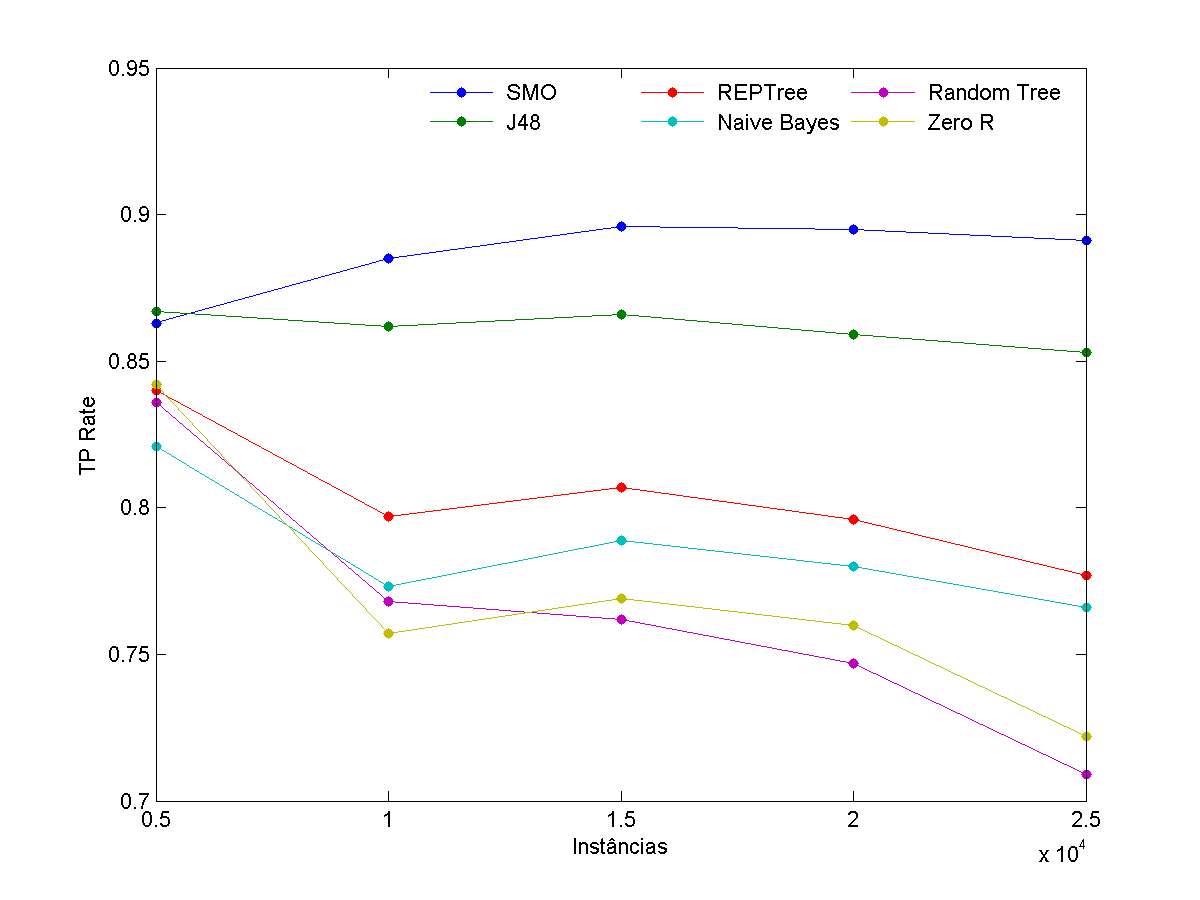
\includegraphics[scale=0.8]{graphs/tp_graph.png}
	\end{center}
	Fonte: Próprio Autor.
\end{figure}

\newpage
Na Figura \ref{figfpRate}, pode confirmar que os algoritmos com melhor desempenho \textit{SMO} e \textit{J48} mostrados na Figura \ref{figtpRate}, apresentam menor \textit{taxa de falso positivo} e com isso um menor custo no processo de classificação de novas instâncias, pois estes algoritmos obtiveram menor quantidade de erros nos \textit{datasets} utilizados.
\\
\begin{figure}[!htb]
	\caption{\label{figfpRate} FP Rate}
	\begin{center}
		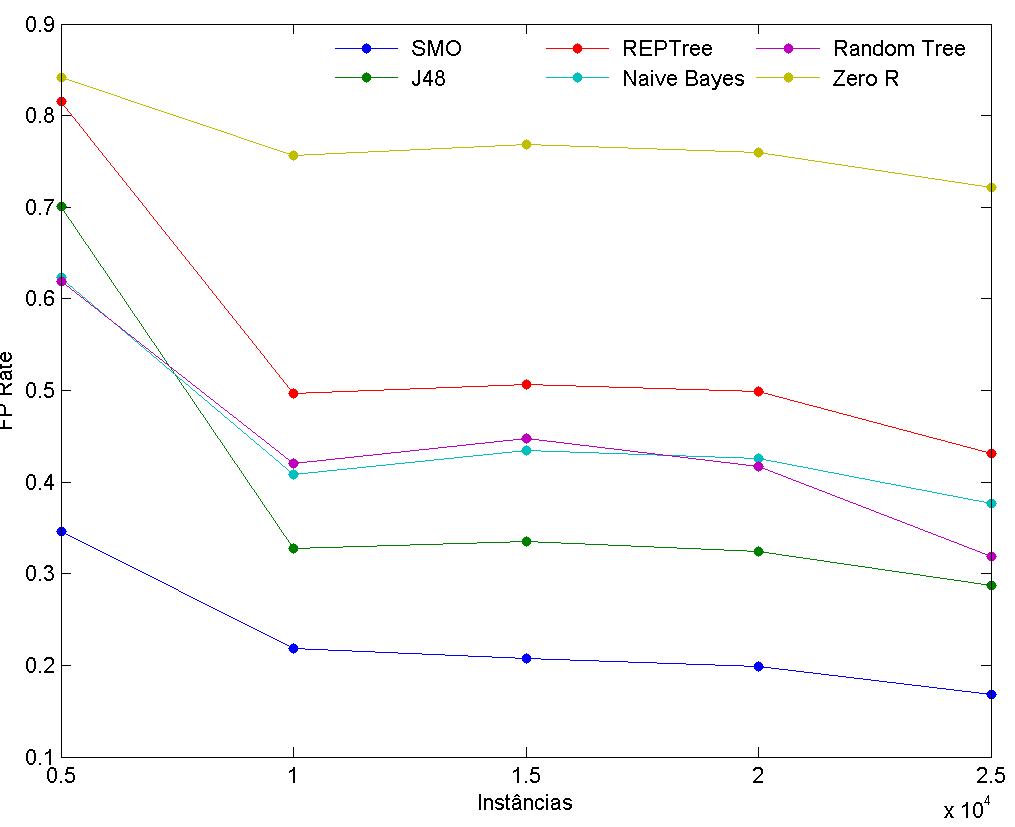
\includegraphics[scale=0.8]{graphs/fp_graph.png}
	\end{center}
	Fonte: Próprio Autor.
\end{figure}
	
	\begin{comment}
	Como podemos observar na Figura \ref{figinstanciasClassificadasCorretamente}, os modelos com melhores resultados SMO e J48.
	\\
	\begin{figure}[!htb]
		\caption{\label{figinstanciasClassificadasCorretamente} Instâncias Classificadas Corretamente}
		\begin{center}
			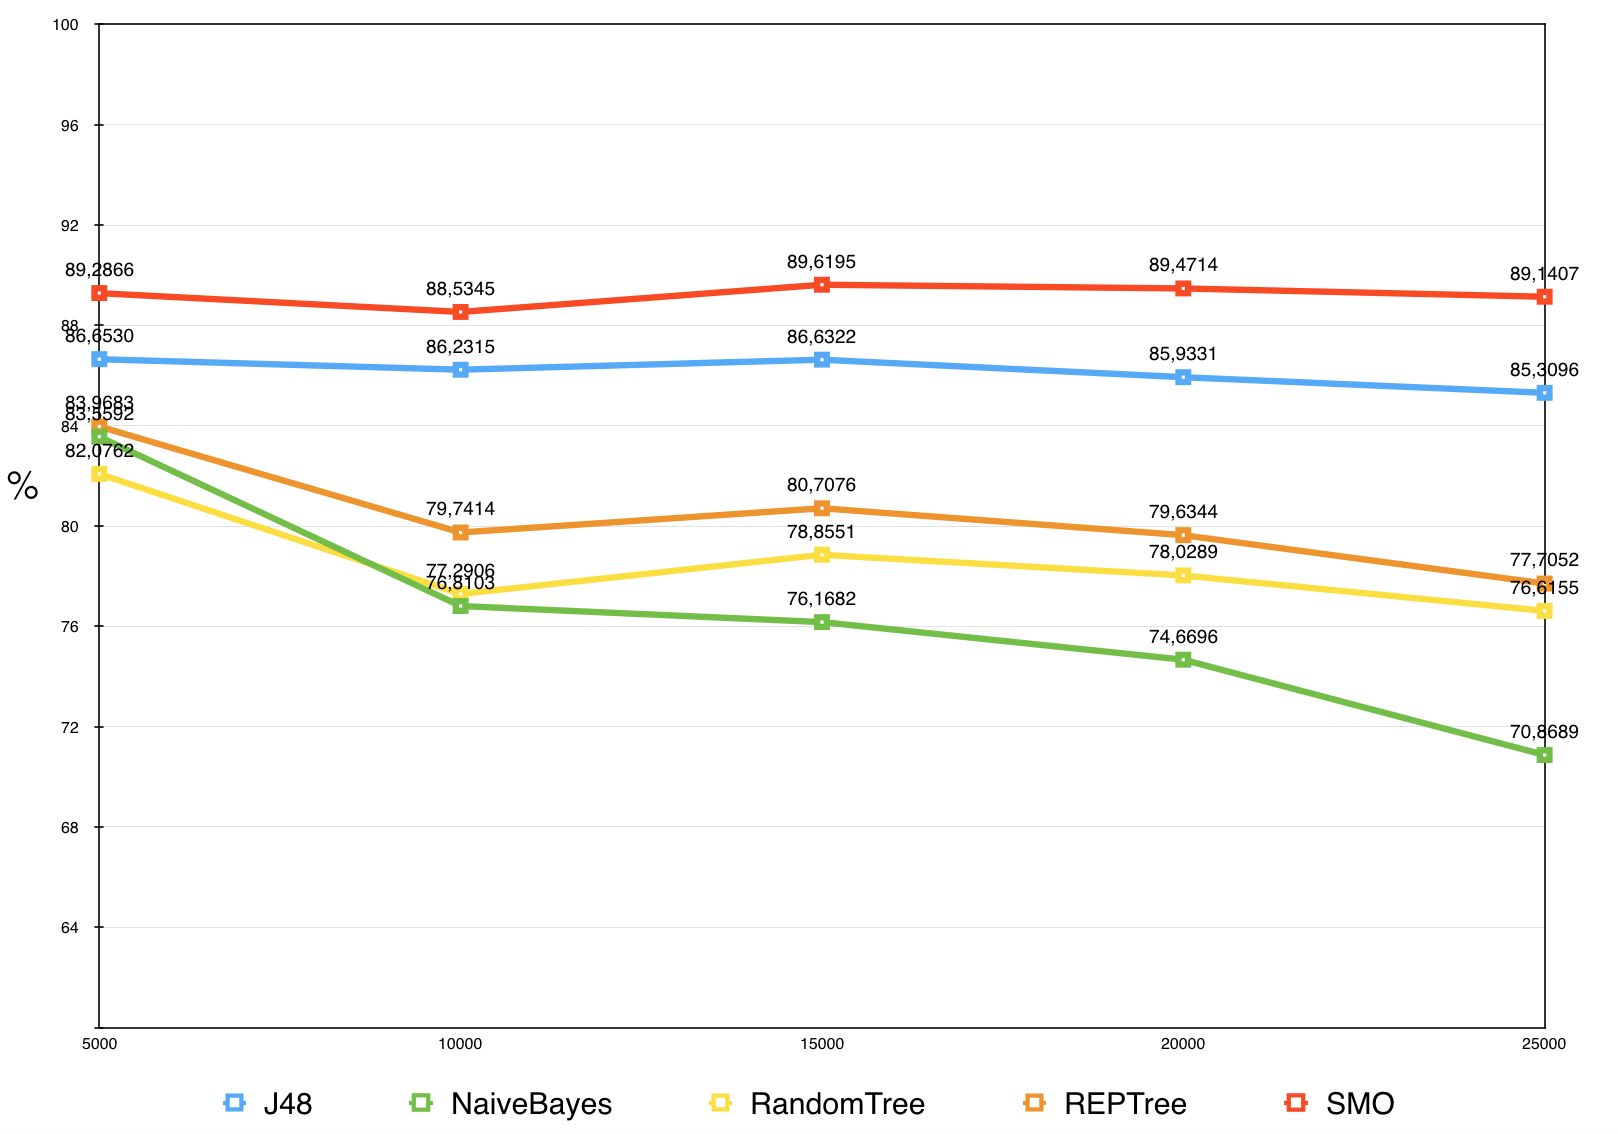
\includegraphics[scale=0.60]{img/instanciasClassificadasCorretamente.png}
		\end{center}
		 Fonte: Próprio Autor.
	\end{figure}
	\end{comment}
	
% - - -
% Capítulo 4
% - - -
\chapter{Conclusões e Trabalhos Futuros}

	Neste Capítulo, apresentado as conclusões do nosso trabalho, incluindo suas limitações  e futuros estudos que possam ser explorados. 

	\section{Resultados Obtidos}

	O Objetivo deste estudo foi construir modelos de classificação por meio do uso de técnicas em \textit{Data Mining} conhecidas como: \textit{Árvore de Decisão}, \textit{Teorema de Bayes} e \textit{Máquinas de Vetores de Suporte}. Estas técnicas foram aplicadas por meio dos algoritmos: \textit{SMO}, \textit{J48}, \textit{REPTree}, \textit{RandomTree} e \textit{NaiveBayes}.
	
	Observando a Figura \ref{figAcertosErrosClassificacao}, pode-se verificar que em todos os conjuntos de dados utilizados nos experimentos, os algoritmos \textit{SMO} e \textit{J48} se destacam em relação aos demais. Com isso os modelos de classificação gerados por esses algoritmos se desempenharam com índices próximos a 90\% no quesito predição de novas instâncias.

	Em \cite{prati:2008}, gráfico ROC(\textit{Receiver Operating Characteristic}) é um método para avaliação e seleção de sistemas de diagnóstico e/ou predição. O gráfico ROC é baseado na probabilidade de detecção ou \textit{taxa de verdadeiros positivos}, e na probalidade de falsos alarmes, ou \textit{taxa de falsos positivos}.
	
	Como pode-se observar na Figura \ref{figTodosModelos}, os modelos gerados pelo algoritmos \textit{SMO} e \textit{J48} obtiveram melhor qualidade, pois se aproximam do ponto $(0,1)$.  Em \cite{prati:2008}, resultados pertecentes ao canto superior esquerdo representam classificadores que possuem melhor desempenho.

	
	\begin{comment}
	\begin{figure}[!htb]
		\caption{\label{figperHits5k} Índice de Classificação - 5K Instâncias}
		\begin{center}
			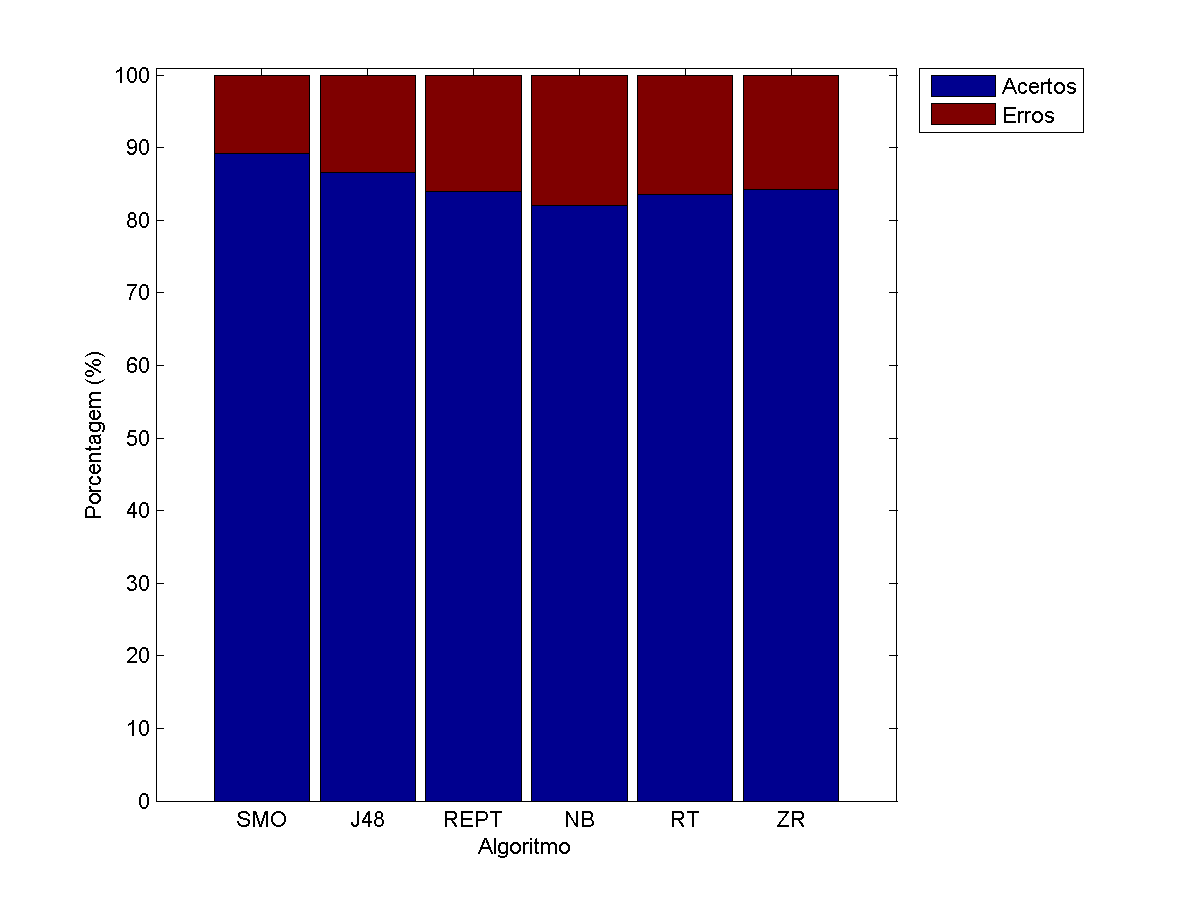
\includegraphics[scale=0.8]{graphs/perc_hits_5k.png}
				Fonte: Próprio Autor.
		\end{center}
	\end{figure}
	\end{comment}
	
	\begin{figure}[!htb]
		\begin{center}
			\caption{\label{figAcertosErrosClassificacao} Gráficos de Acertos e Erros de Classificação}
		\end{center}
		\subfigure[5k Instâncias\label{surreal1}]{
		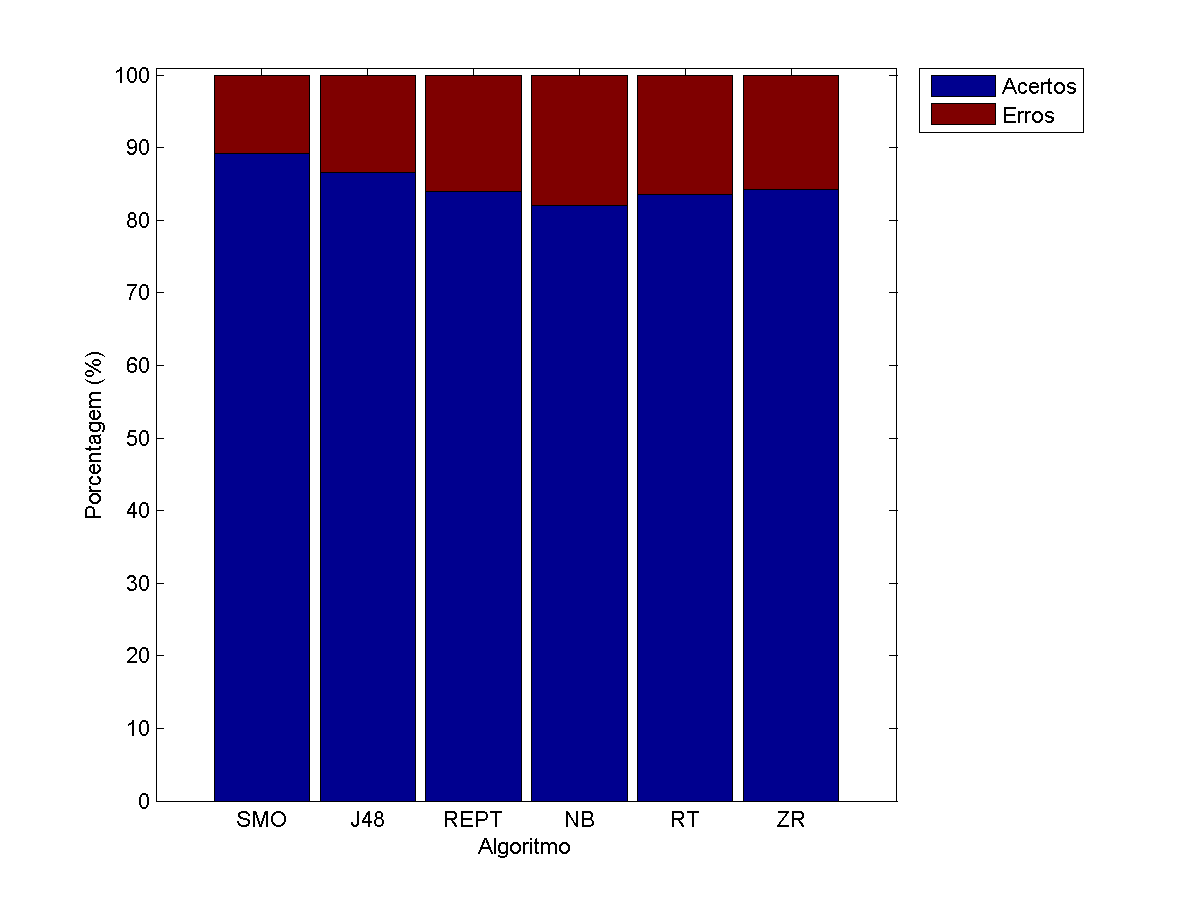
\includegraphics[width=08.5cm, height=07cm]{graphs/perc_hits_5k.png}}
		\subfigure[10k Instâncias\label{surreal2}]{
		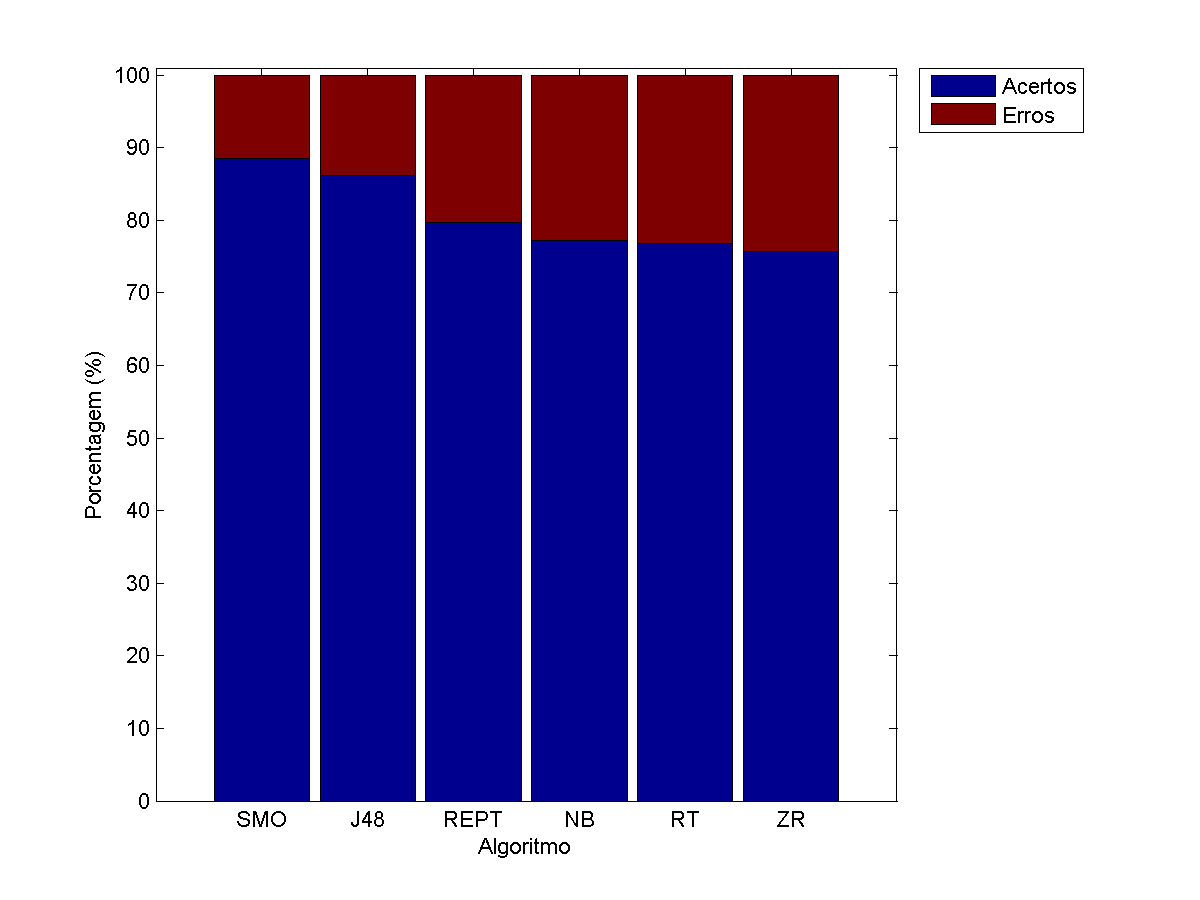
\includegraphics[width=08.5cm, height=07cm]{graphs/perc_hits_10k.png}}
		\subfigure[15k Instâncias\label{surreal3}]{
		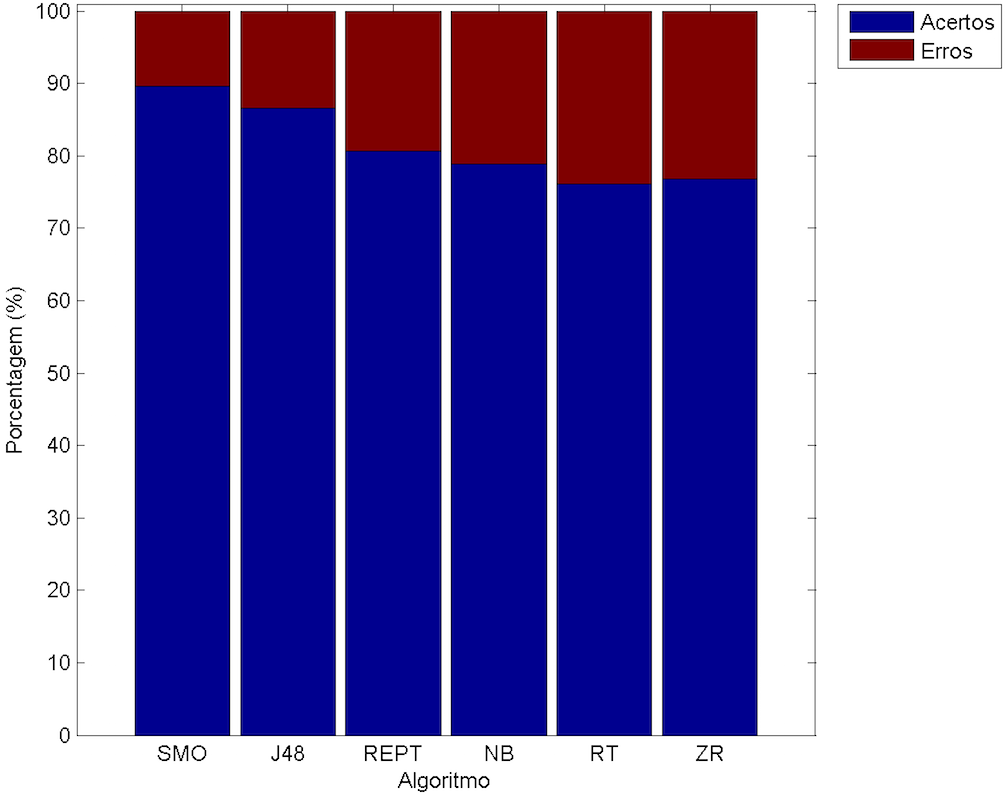
\includegraphics[width=08.5cm, height=07cm]{graphs/perc_hits_15k.png}}
		\subfigure[20k Instâncias\label{surreal4}]{
		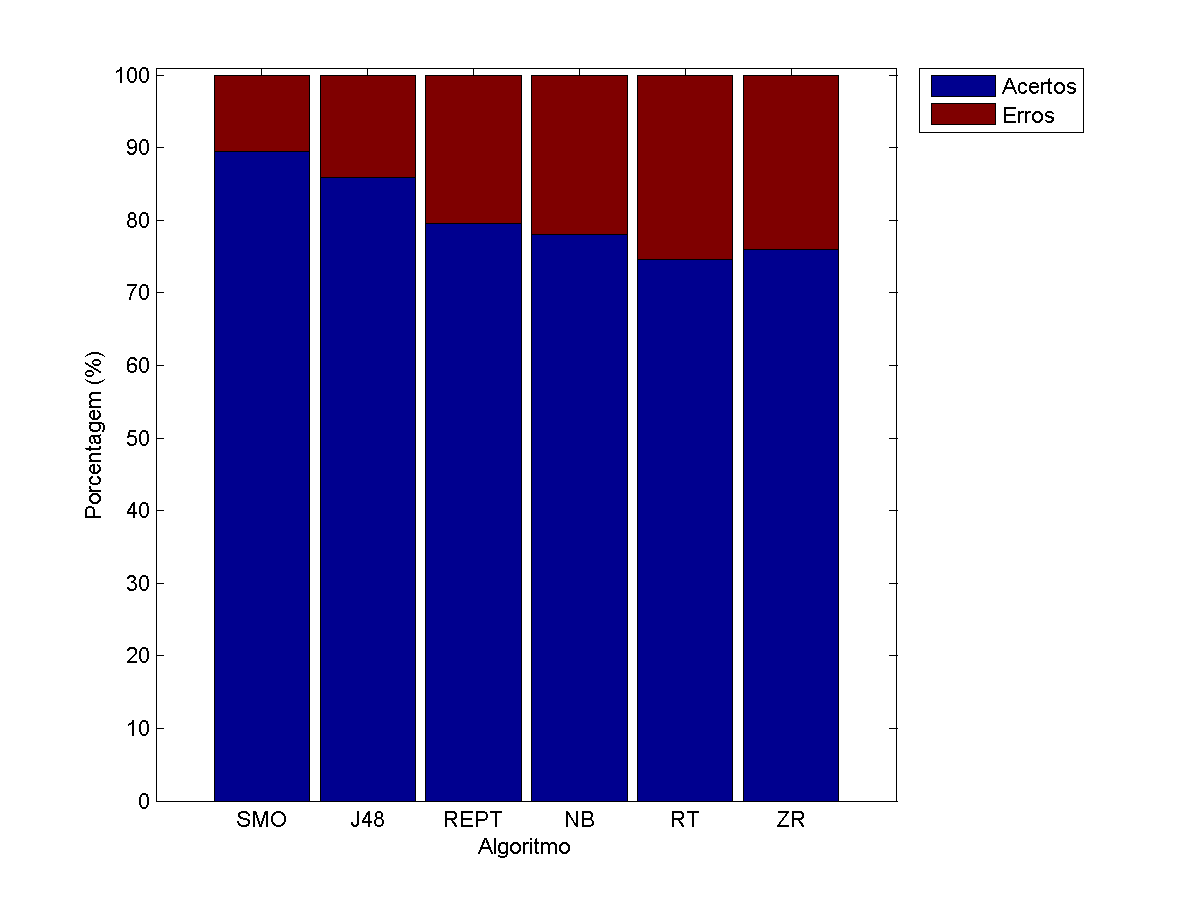
\includegraphics[width=08.5cm, height=07cm]{graphs/perc_hits_20k.png}}
		\begin{center}
		\subfigure[25k Instâncias\label{surreal5}]{
		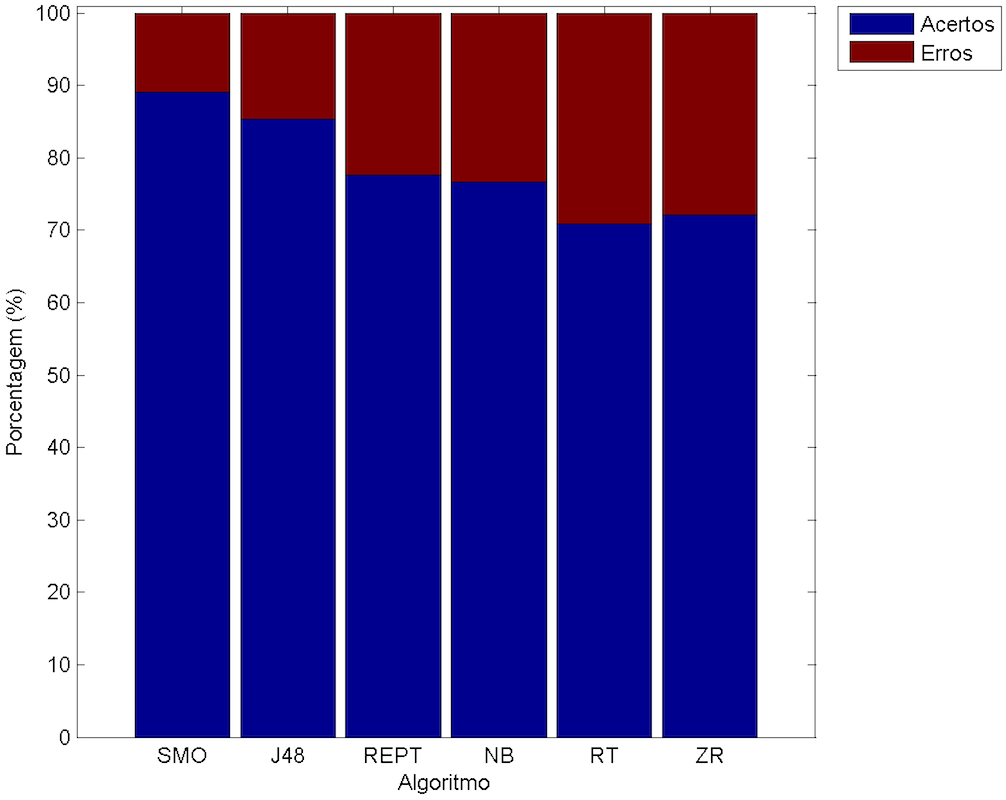
\includegraphics[width=08.5cm, height=07cm]{graphs/perc_hits_25k.png}}
		\end{center}
	\end{figure}

	\begin{comment}

	\begin{figure}[!htb]
		\caption{\label{figperHits10k} Índice de Classificação - 10K Instâncias}
		\begin{center}
			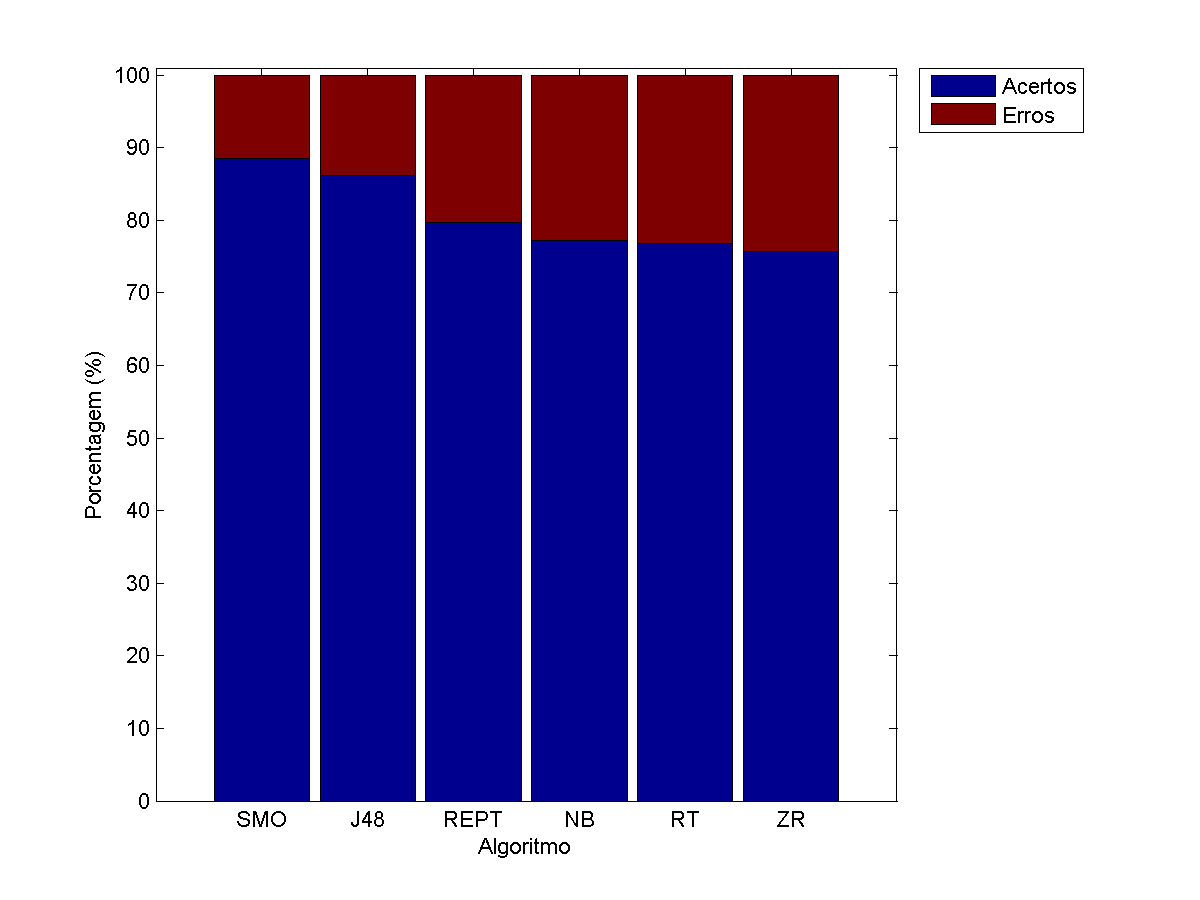
\includegraphics[scale=0.8]{graphs/perc_hits_10k.png}
		\end{center}
		Fonte: Próprio Autor.
	\end{figure}
	
	\pagebreak
	\clearpage
	\newpage
	
	\begin{figure}[!htb]
		\caption{\label{figperHits15k} Índice de Classificação - 15K Instâncias}
		\begin{center}
			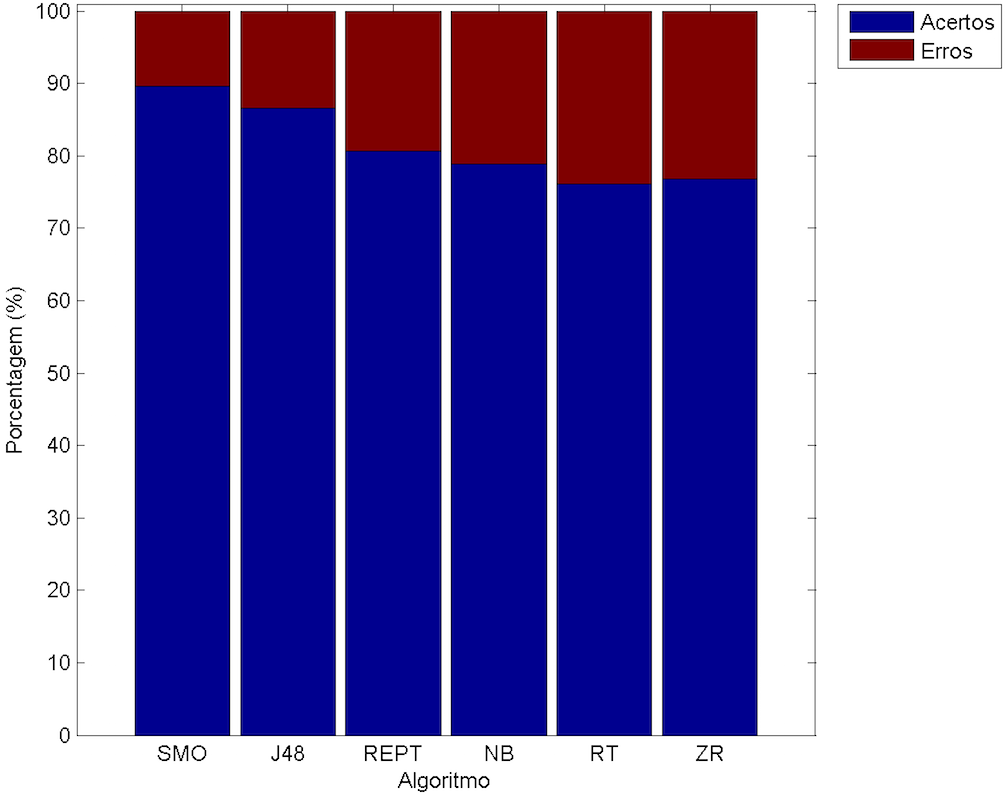
\includegraphics[scale=0.8]{graphs/perc_hits_15k.png}
			Fonte: Próprio Autor.
		\end{center}
	\end{figure}
	
	\begin{figure}[!htb]
		\caption{\label{figperHits20k} Índice de Classificação - 20K Instâncias}
		\begin{center}
			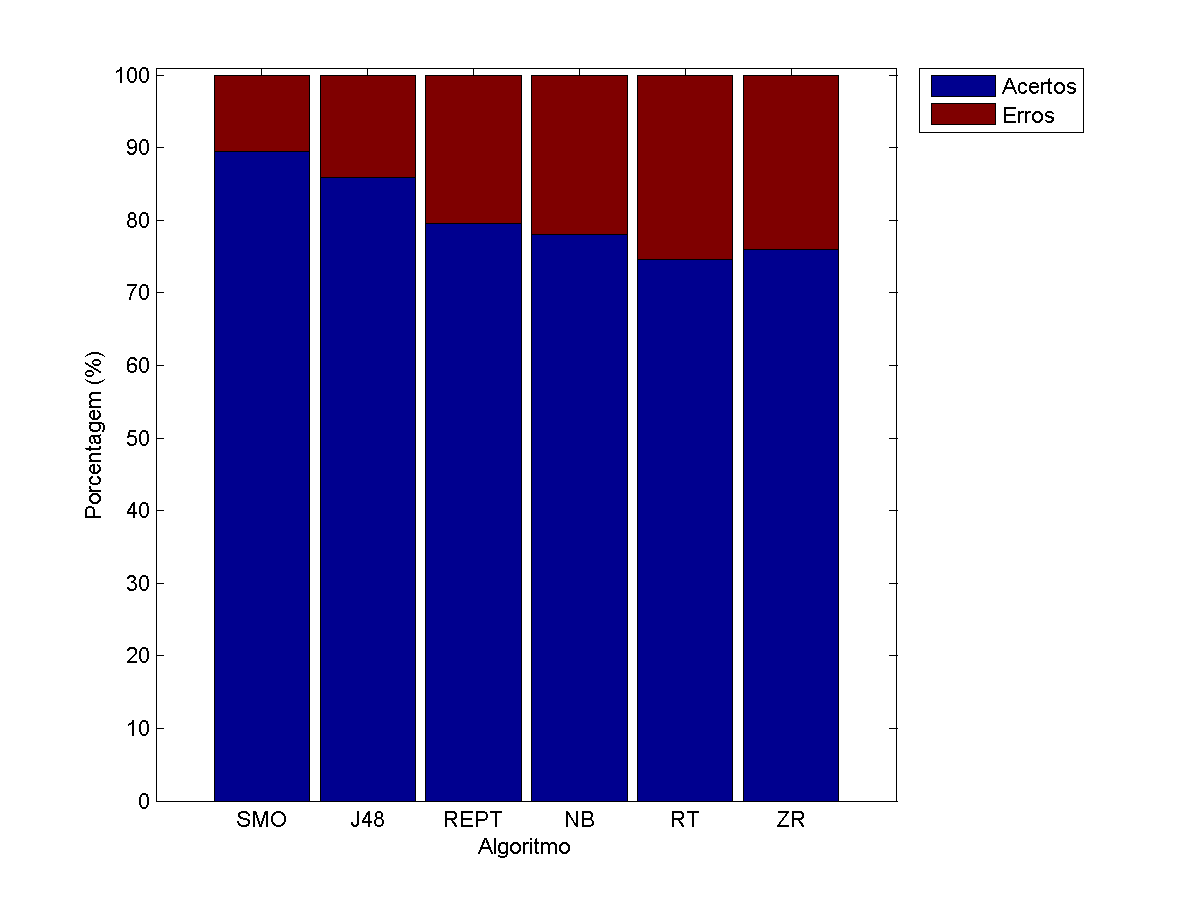
\includegraphics[scale=0.8]{graphs/perc_hits_20k.png}
			Fonte: Próprio Autor.
		\end{center}
	\end{figure}
	
	\pagebreak
	\clearpage
	\newpage
	
	
	\begin{figure}[!htb]
		\caption{\label{figperHits25k} Índice de Classificação - 25K Instâncias}
		\begin{center}
			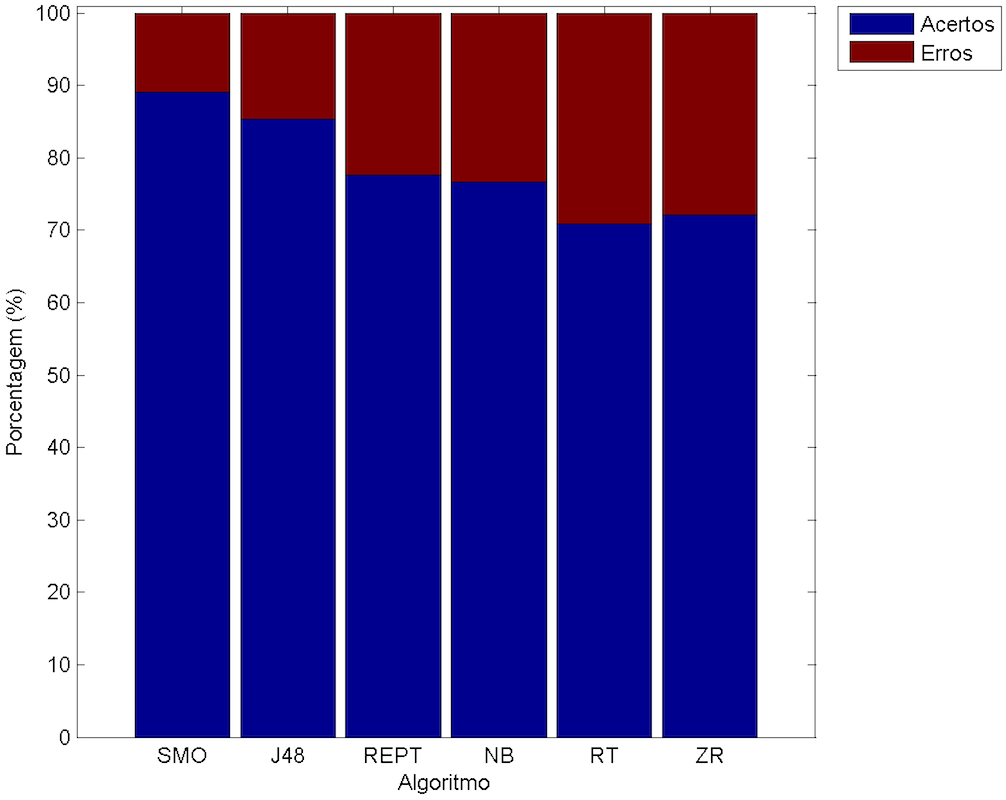
\includegraphics[scale=0.8]{graphs/perc_hits_25k.png}
			Fonte: Próprio Autor.
		\end{center}
	\end{figure}
	\end{comment}
	
	\pagebreak
	\clearpage
	\newpage
	\begin{figure}[!htb]
		\caption{\label{figTodosModelos} Modelos de Classificação no Espaço ROC}
		\begin{center}
			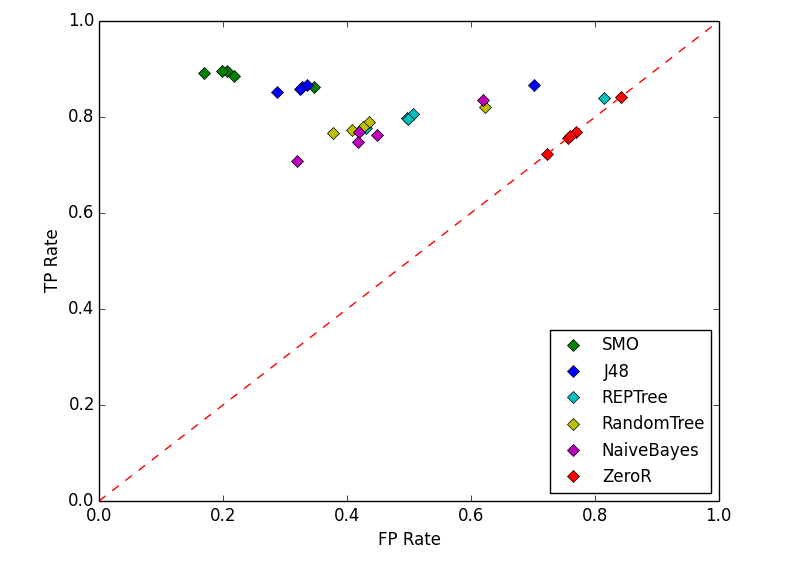
\includegraphics[scale=0.8]{python/TodosModelos.png}
		\end{center}
		Fonte: Próprio Autor.
	\end{figure}

	\begin{comment}
	\begin{figure}[!htb]
		\caption{\label{figRocSMO} Gráfico ROC - Algoritmo SMO}
		\begin{center}
			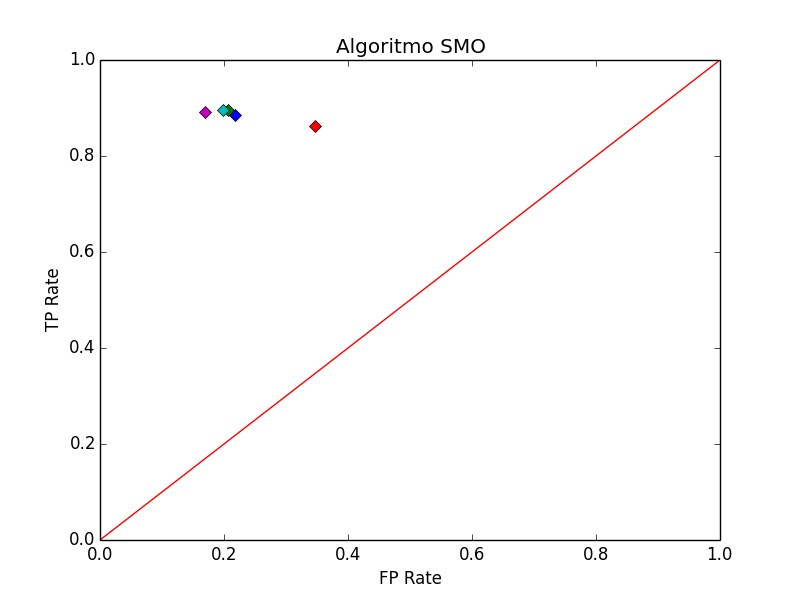
\includegraphics[scale=0.8]{python/smo.png}
			Fonte: Próprio Autor.
		\end{center}
	\end{figure}
	
	\pagebreak
	\clearpage
	\newpage
	
	
	\begin{figure}[!htb]
		\caption{\label{figRocJ48} Gráfico ROC - Algoritmo J48}
		\begin{center}
			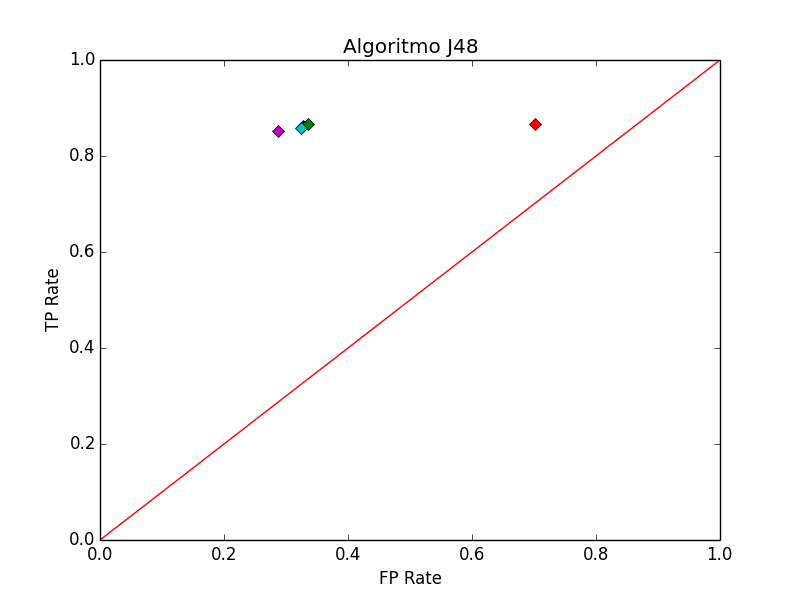
\includegraphics[scale=0.8]{python/j48.png}
			Fonte: Próprio Autor.
		\end{center}
	\end{figure}
	
	\begin{figure}[!htb]
		\caption{\label{figRocRandomTree} Gráfico ROC - Algoritmo RandomTree}
		\begin{center}
			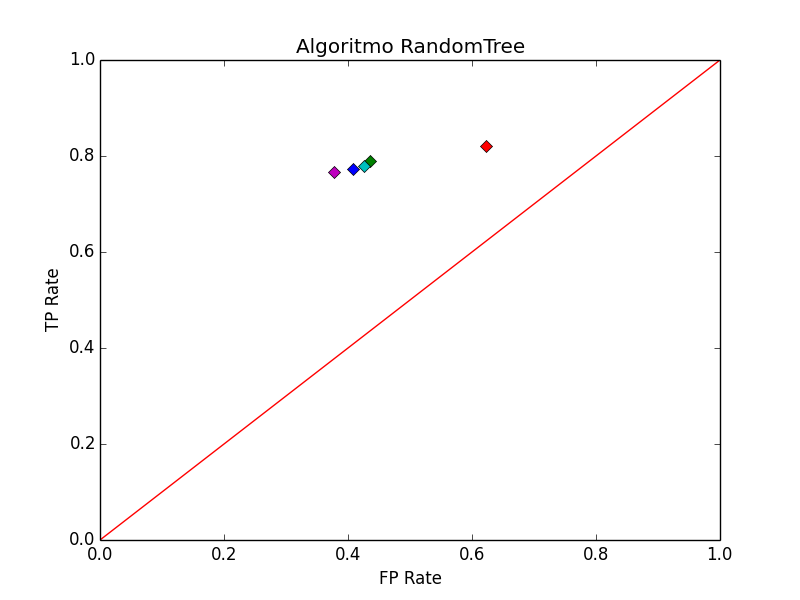
\includegraphics[scale=0.8]{python/RandomTree.png}
			Fonte: Próprio Autor.
		\end{center}
	\end{figure}
	
	\pagebreak
	\clearpage
	\newpage
	
	
	\begin{figure}[!htb]
		\caption{\label{figRocREPTree} Gráfico ROC - Algoritmo REPTree}
		\begin{center}
			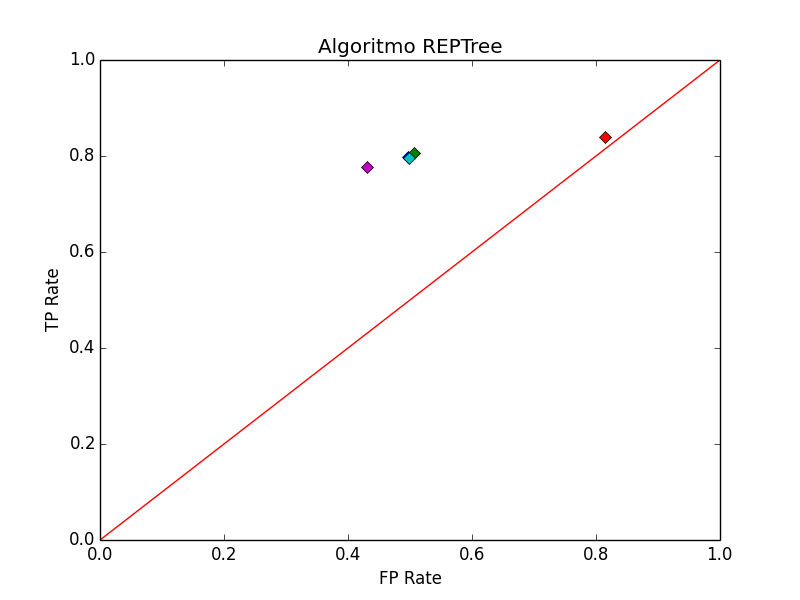
\includegraphics[scale=0.8]{python/REPTree.png}
			Fonte: Próprio Autor.
		\end{center}
	\end{figure}
	
	\begin{figure}[!htb]
		\caption{\label{figRocNaiveBayes} Gráfico ROC - Algoritmo NaiveBayes}
		\begin{center}
			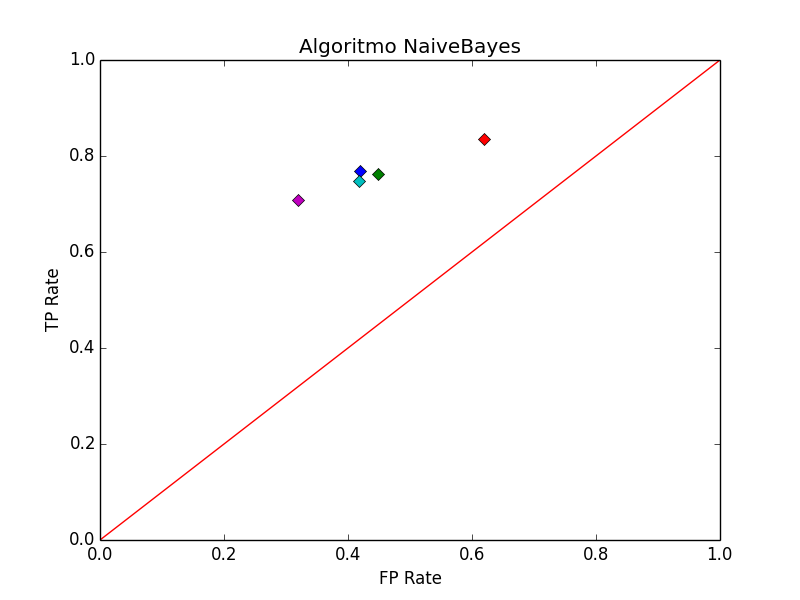
\includegraphics[scale=0.8]{python/NaiveBayes.png}
			Fonte: Próprio Autor.
		\end{center}
	\end{figure}
	
	\pagebreak
	\clearpage
	\newpage
	
	
	\begin{figure}[!htb]
		\caption{\label{figRocZeroR} Gráfico ROC - Algoritmo ZeroR}
		\begin{center}
			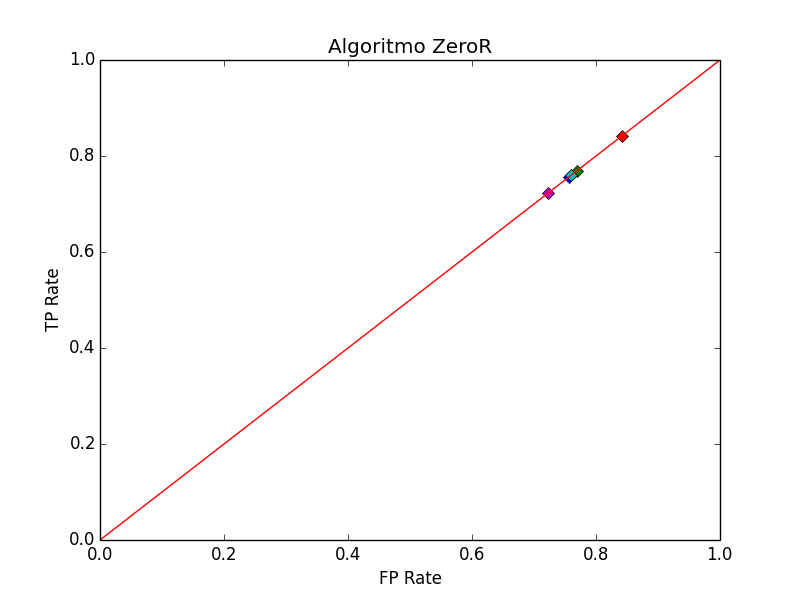
\includegraphics[scale=0.8]{python/ZeroR.png}
			Fonte: Próprio Autor.
		\end{center}
	\end{figure}
	\end{comment}
	
	\section{Trabalhos Futuros}
	
	Como trabalhos futuros, podem ser explorados na continuação desta pesquisa as oportunidades descritas a seguir:
	
	\begin{itemize}
		\item Implementar remoção de instâncias que influenciam na qualidade do classificador.
		\item Adaptar a construção de modelos em tempo real.
		\item Integrar informações de precipitação de chuva da região onde os dados foram coletados.
		\item Usar outros algoritmos de classificação.
	\end{itemize}

% ----------------------------------------------------------
% ELEMENTOS PÓS-TEXTUAIS
% ----------------------------------------------------------
\postextual
\Spacing{1.5}
% -----------------------------------------------------------------------------
% Referencias Bibliograficas
% -----------------------------------------------------------------------------
%\bibliographystyle{abnt-alf}
\bibliography{referencias}

% ----------------------------------------------------------
% Apêndices
% ----------------------------------------------------------

% ---
% Inicia os apêndices
% ---

%\begin{apendicesenv}

% ----------------------------------------------------------
%\chapter{Primeiro apêndice}
% ----------------------------------------------------------

%Os apêndices são textos ou documentos elaborados pelo autor, a fim de complementar sua argumentação, sem prejuízo da unidade nuclear do trabalho.

%\end{apendicesenv}

% Anexos
% ----------------------------------------------------------

% ---
% Inicia os anexos
% ---
\begin{anexosenv}

% ---
%\chapter{Dicionário de dados - SINAN online}

%Este anexo descreve todos os atrubutos presentes no SINAN
% ---

%inserindo todas as páginas
%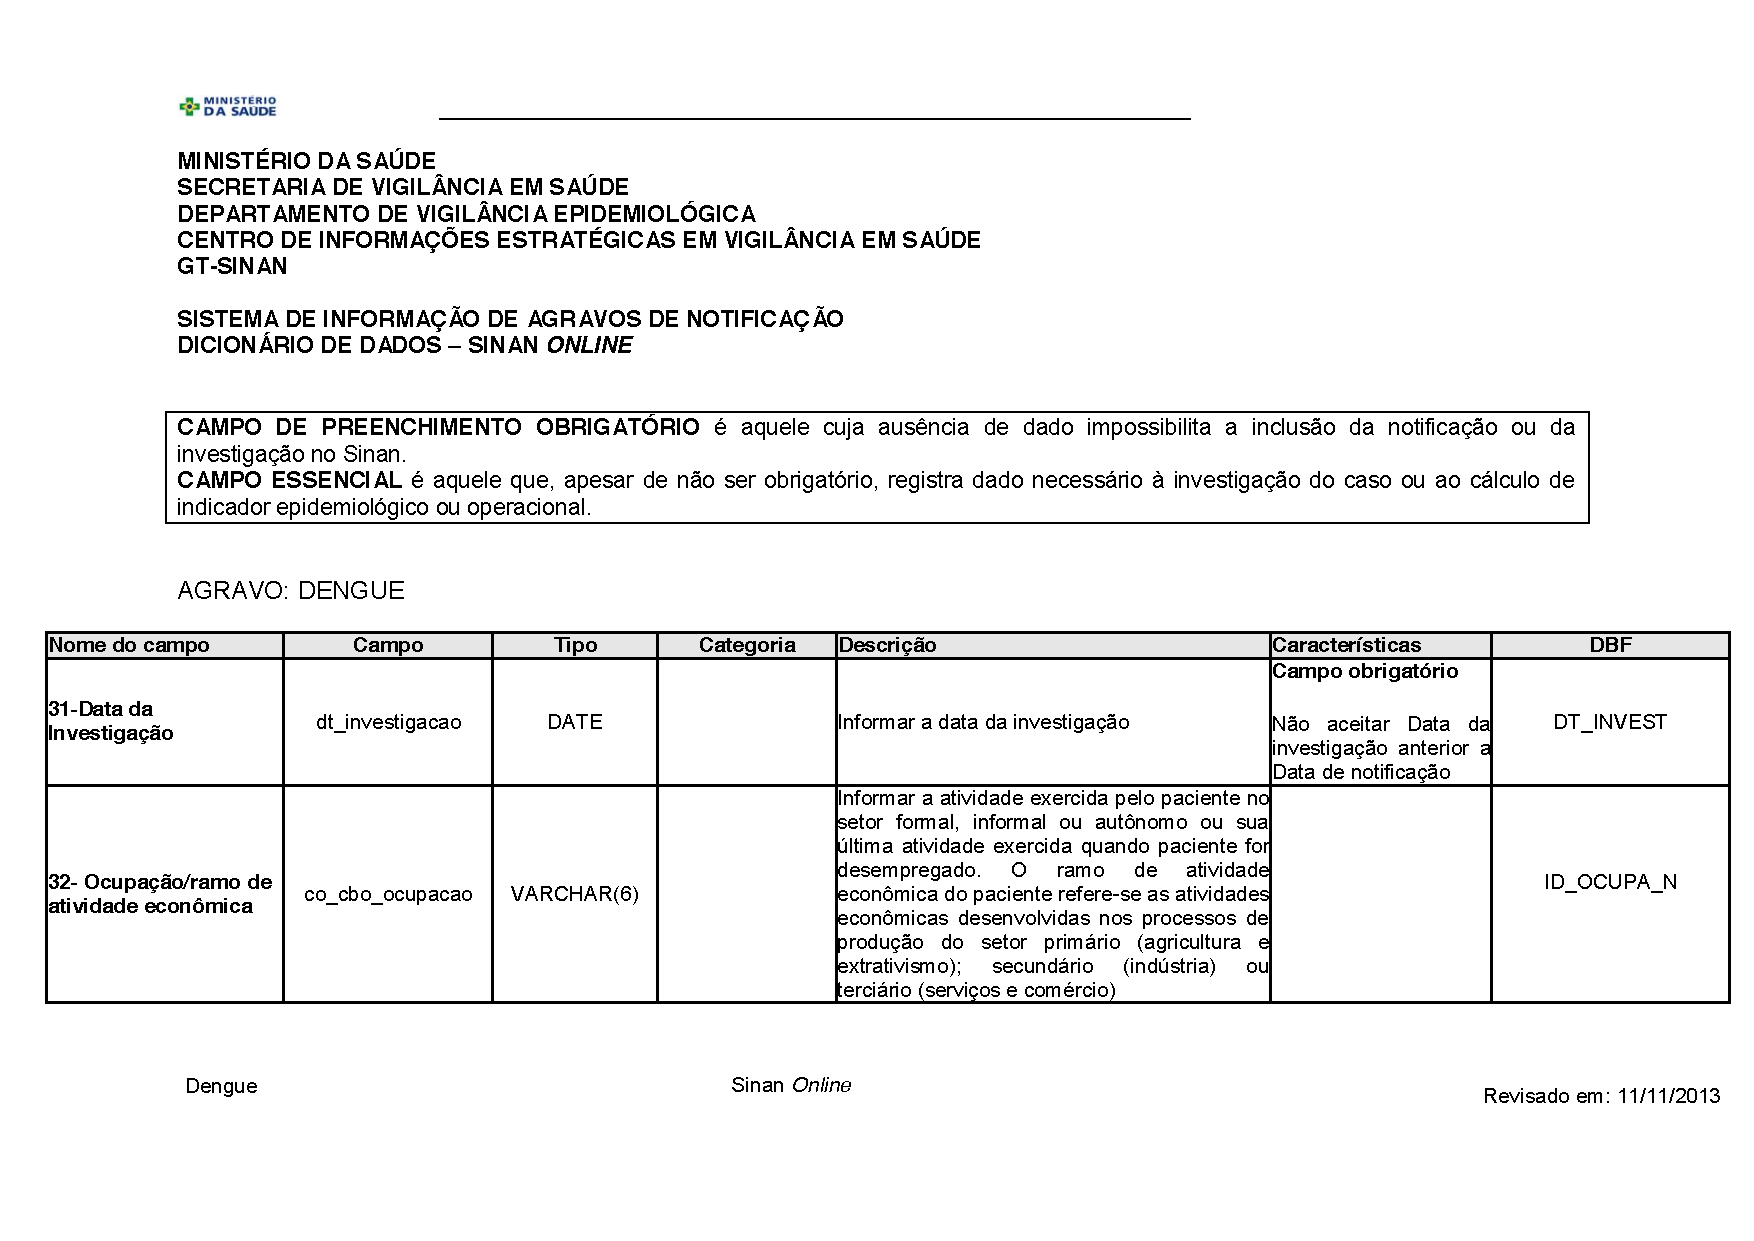
\includepdf[pages=-,landscape]{files/dicionarioDados.pdf}

\end{anexosenv}

\end{document}